\documentclass[12pt, a4paper]{article}
\usepackage[bottom=2cm,top=3cm,left=2cm,right=2cm]{geometry}
\usepackage[portuguese]{babel}
\usepackage[utf8]{inputenc}
\usepackage{CJKutf8}
\usepackage{mathtext}
\usepackage{wrapfig}
\usepackage[T1]{fontenc}
\usepackage{blindtext}
\usepackage{tasks}
\usepackage{setspace}
\usepackage{verbatim}
\usepackage[dvipsnames]{xcolor}

%\usepackage{tikz}
\usepackage{tikz-cd}%Para diagramas 
\usepackage[framemethod=Tikz]{mdframed}
\usepackage{amsmath}
\usepackage{amsfonts}
\usepackage{amssymb}
\usepackage{wasysym}
\usepackage{amsthm}
\usepackage{graphics}
\usepackage{pifont}
\usepackage{arydshln} %dashed line nas matrizes
%\usepackage{lipsum}
%\usepackage{CJKutf8} %Pacote para escrever em japonês \begin{CJK}{UTF8}{min} \end{CJK}
\usepackage{multicol}
\usepackage{wasysym}
% \usepackage{colorspace}
\usepackage[arrow,matrix,curve]{xy}
\usepackage{enumitem}
\usepackage{graphicx, color}
%\usepackage{eulervm} %Fonte de texto
\usepackage{exsheets} %Mostrar soluções
\usepackage{commath}
\usepackage{mathpazo}
\usepackage{cancel}
%-------------------------------------------------------------
%Comandos úteis
\newcommand{\mdc}{{\rm mdc}}
\newcommand{\mmc}{{\rm mmc}}
\newcommand{\sen}{{\rm sen}}
\newcommand{\tg}{{\rm tg}}
\newcommand{\cotg}{{\rm cotg}}
\newcommand{\cossec}{{\rm cossec}}
\newcommand{\arctg}{{\rm arctg}}
\newcommand{\arcsen}{{\rm arcsen}}
\newcommand{\negrito}[1]{\mbox{\boldmath{$#1$}}} 
\newcommand{\heart}{\ensuremath\heartsuit}
\newcommand{\diamonde}{\ensuremath\diamondsuit}
\newtheorem{defi}{Definição}
\newtheorem{prop}{Proposição}
\newtheorem{dem}{Demonstração}
\newtheorem{coro}{Corolário}
\DeclareSymbolFont{extraup}{U}{zavm}{m}{n}
\DeclareMathSymbol{\varheart}{\mathalpha}{extraup}{86}
\DeclareMathSymbol{\vardiamond}{\mathalpha}{extraup}{87}
\setlength{\parindent}{0pt}
\newcommand{\tn}[1]{\textnormal{#1}} 
\newcommand{\Hom}{\tn{Hom}}
\newcommand{\End}{\tn{End}}
\newcommand{\Z}{\mathbb{Z}}
\newcommand{\R}{\mathbb{R}}
\renewcommand{\rmdefault}{ptm} 
\newcommand{\spec}{\textrm{Spec}}

%-------------------------------------------------------------
%Boxes para critérios de correção, caso seja necessário

%Alternativa Verde e azul para avisos    
    \mdfdefinestyle{Criterios}{%
    linecolor=blue,
    outerlinewidth=2pt,
    roundcorner=10pt,
    innertopmargin=\baselineskip,
    innerbottommargin=\baselineskip,
    innerrightmargin=20pt,
    innerleftmargin=20pt,
    backgroundcolor=white!75!green}
    
%Box padrão    
\mdfdefinestyle{MyFrame}{%
    linecolor=blue,
    outerlinewidth=2pt,
    roundcorner=20pt,
    innertopmargin=\baselineskip,
    innerbottommargin=\baselineskip,
    innerrightmargin=20pt,
    innerleftmargin=20pt,
    backgroundcolor=white!50!white}
    
%\mdfdefinestyle{Solução}{%
%    linecolor=blue,
%    outerlinewidth=1pt,
%    roundcorner=8pt,
%    innertopmargin=4pt%\baselineskip,
%    innerbottommargin=0pt%\baselineskip,
%    innerrightmargin=20pt,
%    innerleftmargin=20pt,
%    backgroundcolor=white!50!white}
    
%Alternativa Verde e azul para avisos    
    \mdfdefinestyle{Aviso}{%
    linecolor=blue,
    outerlinewidth=2pt,
    roundcorner=20pt,
    innertopmargin=\baselineskip,
    innerbottommargin=\baselineskip,
    innerrightmargin=20pt,
    innerleftmargin=20pt,
    backgroundcolor=white!50!green}
    
%----------------------------------------------------------------
%Cores do documento
\definecolor{Floresta}{rgb}{0.13,0.54,0.13}    
% \definespotcolor{mygreen}{PANTONE 7716 C}{.83, 0, .00, .51}
% \definespotcolor{tuti}{}{0.6, 0, 1, .508}

%----------------------------------------------------------------
%Uso de counters para numeração automática dos exercícios 
%Para mais infos: https://www.overleaf.com/learn/latex/Counters

\newcounter{exercicio}[section]
\newenvironment{exercicio}[1][]{\refstepcounter{exercicio}\par\medskip
 \textcolor{blue}{\bf(\theexercicio)} \rmfamily}{\medskip }
   
 \usepackage{ifmtarg}% http://ctan.org/pkg/ifmtarg
 
 \makeatletter 
 \newcommand{\isempty}[1]{%
  \@ifmtarg{#1}{\begin{question}}{\begin{question}[topic=#1]}}

% \newcommand{\isempty}[1]{%
%  \@ifmtarg{#1}{\begin{question}}{\begin{question}[topic=#1]}}
  
    
 
 
\newenvironment{solucao}[1][]{\textbf{\\ \\ \textcolor{red}{Solução:}}#1 \rmfamily}{\medskip }


\newenvironment{criterios}[1][]{
 \textcolor{blue}{\bf Critérios de Correção:} \rmfamily \par\medskip #1 }{\medskip }
 
\newcommand{\itens}[1]{\begin{tasks}[label={(tsk[a])},label-width=3.6ex, label-format = {\bfseries}, column-sep = {0pt}](1) #1\end{tasks}}

\newcommand{\itensladoalado}[2]{\begin{tasks}[label={(tsk[a])},label-width=3.6ex, label-format = {\bfseries}, column-sep = {0pt}](#1) #2 \end{tasks}}

\newcommand{\alt}[1]{\textcolor{Floresta}{$\negrito{(#1)} $}}

%\newcommand{\alt}[1]{\task[\pers{#1}]}

%\newcommand{\solucao}[1]{
%\textbf{\\ \\ \textcolor{red}{Solução:}} #1}

%----------------------------------------------------------------
%Dados da lista:

\newcommand{\titulo}{MAT0120 - Álgebra I para Licenciatura}
\newcommand{\lista}{Lista 1}
\newcommand{\professor}{Kostiantyn Iusenko}
\newcommand{\monitor}{Douglas de Araujo Smigly}
\newcommand{\semestre}{1º Semestre de 2021}
%----------------------------------------------------------------

%Mostrar ou não as soluções
%\SetupExSheets{solution/print=true} %Se print=false, este arquivo Não imprime as soluções.
\SetupExSheets{solution/print=true}


%Solução sem numeração (pois vem logo depois da questão) - se quiser com números, basta comentar os comandos abaixo:
\DeclareInstance{exsheets-heading}{block-no-nr}{default}{
  attach = {
    main[l,vc]title[l,vc](0pt,0pt) ;
    main[r,vc]points[l,vc](\marginparsep,0pt)
  }
}

%  {question}[headings=block-subtitle] - por bloco
\RenewQuSolPair
  {question}[headings=block-no-nr]
  {solution}[headings=block-no-nr]

%Personalização de Questão/ Solução
\SetupExSheets{
  counter-format=se.qu.,
  question/name= ,
  solution/name=\textcolor{red}{Solução}
}

%Cabeçalho
%----------------------------------------------------------------
\title{\vspace{-15mm}\fontsize{16pt}{10pt}\selectfont\textbf{\titulo} \\ \vspace{5mm} \textbf{\textcolor{Floresta}{\lista}} \PrintSolutionsT{ - \textcolor{blue}{Soluções}}} % Article title
%\title{\fontsize{16pt}{10pt}{\textbf{MAT0501/MAT6680 - Tópicos de Anéis e Módulos}}
\author{Professor: \professor \\ Monitor: \monitor}
\date{\semestre}
\begin{document}
\maketitle
%------------------------------------------------------------
%Caso queira multicols, só descomentar as linhas abaixo 
%e lembrar de colocar \end{multicols*} no final do documento
%e columnbreak se quiser criar uma nova coluna

%\begin{multicols*}{2}
%\setlength{\columnseprule}{0.78pt}
%\raggedcolumns
%\columnbreak
%------------------------------------------------------------

%------------------------------------------------------------
%
% Exemplos de exercícios:
%
%------------------------------------------------------------
\section{Axiomática de $\mathbb{Z}$}
%Questão simples
\begin{exercicio}
Dado um inteiro $x,$ chamamos de \textit{valor absoluto} de $x$ o numero inteiro designado por $\abs{x}$ e definido por
\[
\abs{x} = \begin{cases}
x, & \mbox{se } x \ge 0 \\
-x, & \mbox{se } x < 0
\end{cases}.
\]
Sejam $a, b \in \mathbb{Z}.$ Prove que
\itens{
\task[\alt{a}] $\abs{a} \ge 0;$
\task[\alt{b}] $\abs{a} = 0$ se, e somente se, $a = 0;$
\task[\alt{c}] $- \abs{a} \le a \le \abs{a};$
\task[\alt{d}] $\abs{ab} = \abs{a} \abs{b};$
\task[\alt{e}] $\abs{a + b} \le \abs{a} + \abs{b};$
\task[\alt{f}] $\abs{\abs{a} - \abs{b}} \le \abs{a - b}.$

}
\end{exercicio}
\begin{solution}
\itens{
\task[\alt{a}] Pela definição de valor absoluto, temos dois casos a analisar:
\begin{itemize}
    \item $a \ge 0:$ Se $a \ge 0,$ então por definição, $\abs{a} = a \ge 0.$
    \item $a < 0.$ Se $a < 0,$ isso significa que $-a > 0,$ e $\abs{a} = -a > 0.$ 
\end{itemize}
Portanto, concluímos que $\abs{a} \ge 0$ para todo $a.$

\task[\alt{b}] $(\abs{a} = 0 \Rightarrow a = 0):$ Vamos verificar que se $\abs{a} \neq 0,$ então $a \neq 0.$ Veja que, se $a < 0,$ então $-a > 0,$ e $\abs{a} = -a > 0,$ o que implica $a \neq 0.$ Agora, se $a > 0,$ então $\abs{a} = a > 0,$ assim $a \neq 0.$ Logo, $\abs{a} = 0$ apenas para $a = 0.$

$(\abs{a} = 0 \Leftarrow a = 0):$ Por definição, $\abs{0} = 0.$
\task[\alt{c}]} Novamente, vamos dividir a situação em dois casos:
\begin{itemize}
    \item Se $a < 0,$ então $-a > 0$ e $\abs{a} = -a > 0 > a$ e $- \abs{a} = a.$ Logo,
    \[
    - \abs{a} = a < \abs{a}.
    \]
    \item Se $a \ge 0,$ então $\abs{a} = a > 0,$ e $- \abs{a} < 0 < a,$ logo
    \[
    -\abs{a} < a = \abs{a}
    \]
\end{itemize}
Juntando as duas informações, temos
\[
- \abs{a} \le a \le \abs{a}
\]
\itens{
\task[\alt{d}] Vamos primeiramente provar que $\abs{a} = \sqrt{a^2}.$ Observe que:
\begin{itemize}
    \item Se $a = 0,$ então $\abs{a} = 0 = \sqrt{0^2} = \sqrt{a^2}.$ 
    \item Se $a > 0,$ então $\abs{a} = a = \sqrt{a^2}.$
    \item Se $a < 0,$ então $-a > 0.$ Assim, pelo caso anterior, segue que $\abs{-a} = \sqrt{(-a)^2}.$ Agora, por definição, como $-a$ é positivo, então $\abs{-a} = -a = \abs{a}.$ Além disso, $\sqrt{(-a)^2} = \sqrt{a^2}.$ Portanto, \[\abs{a} = \abs{-a} = \sqrt{(-a)^2} = \sqrt{a^2}.\]
    \end{itemize}
    Agora, aplicando tal propriedade na igualdade que precisamos verificar, ficamos com
    \[
    \abs{ab} = \sqrt{(ab)^2} = \sqrt{(a^2b^2)} = \sqrt{a^2} \sqrt{b^2} = \abs{a} \abs{b}.
    \]
    
\task[\alt{e}] Utilizando o item (c), temos:}
\[
- \abs{a} \le a \le \abs{a} \quad \mbox{e} \quad - \abs{b} \le b \le \abs{b}.
\]
Somando ambas, vem
\[
-(\abs{a} + \abs{b}) \le a + b \le \abs{a} + \abs{b}
\]
Vamos agora analisar os possíveis valores de $a+b$ na identidade acima:
\begin{itemize}
    \item Se $a + b \ge 0,$ então $\abs{a + b} = a + b \le \abs{a} + \abs{b}$
    \item Se $a + b < 0,$ então $\abs{a + b} = -(a+b) \le \abs{a} + \abs{b}.$ 
    \end{itemize}
    Em ambos os casos, concluímos que $\abs{a + b} \le \abs{a} + \abs{b}.$
\itens{
\task[\alt{f}] Observe que, pela Desigualdade Triangular provada no item (e)}
\[
\abs{a} = \abs{a-b+b} = \abs{\textcolor{Cyan}{(a-b)} + \textcolor{Red}{b}} \le \abs{\textcolor{Cyan}{a - b}} + \abs{\textcolor{Red}{b}}.
\]
Logo, 
\[
\abs{a} - \abs{b} \le \abs{a - b} + \abs{b} - \abs{b} = \abs{a - b} \Rightarrow \abs{a} - \abs{b} \le \abs{a - b}.
\]
Por outro lado, com o resultado acima, trocando $a$ com $b$, temos $\abs{b} - \abs{a} \le \abs{b - a} $, o que nos permite limitar $-\abs{a - b}$ por
\[
\abs{a - b} = \abs{-(a-b)} = \abs{b - a} \ge \abs{b} - \abs{a} = -(\abs{a} - \abs{b}) \Rightarrow - \abs{a - b} \le \abs{a} - \abs{b}.
\]
Juntando as duas informações, temos:
\[
- \abs{a - b} \le \abs{a} - \abs{b} \le \abs{a - b}.
\]
Vamos analisar os possíveis valores de $\abs{a}-\abs{b}:$
\begin{itemize}
    \item Se $\abs{a} - \abs{b} \ge 0,$ então $\abs{\abs{a} - \abs{b}} = \abs{a} - \abs{b} \le \abs{a-b}.$
    \item Se $\abs{a} - \abs{b} < 0,$ então $\abs{\abs{a} - \abs{b}} = -(\abs{a} - \abs{b}) = \abs{b} - \abs{a} \le \abs{b - a} = \abs{-(a-b)} = \abs{a - b}.$ 
    \end{itemize}
    Em ambos os casos, concluímos que $\abs{\abs{a} - \abs{b}} \le \abs{a-b}.$

\end{solution}
%Questão com alternativas
\begin{exercicio}
Prove que o conjunto $S = \{ m \in \mathbb{Z} \mid 7 < m < 8 \}$ é vazio.
\end{exercicio}
\begin{solution}
Observe que, se $m \in \mathbb{Z}$ é tal que $7 < m < 8,$ então $0 < m - 7 < 1.$ Assim,
\[
S = \{ m \in \mathbb{Z} \mid 7 < m < 8 \} = \{ m \in \mathbb{Z} \mid 0 < m-7 < 1 \},
\]
e tomando $s \in \mathbb{Z},$ basta mostrar que o conjunto 
\[
S^{\prime} =  \{ s \in \mathbb{Z} \mid 0 < s < 1 \}
\]
é vazio. Para isto, vamos supor por absurdo que $S^{\prime} \neq \emptyset.$ Nesse caso, $S^{\prime}$ é um conjunto não-vazio de números inteiros não-negativos, e pelo Princípio da Boa Ordem, segue que este admite um elemento mínimo. Chamemo-lo de $\xi.$ Assim,
\[
\xi \in S \Rightarrow 0 < \xi < 1.
\]
Multiplicando ambos os membros da desigualdade por $\xi$, temos que $0 < \xi^2 < \xi < 1.$ Ou seja, existe um outro elemento $\xi^2 \in S^{\prime}$ que e menor que $\xi$, o que é absurdo, pois $\xi$ é minimal. Logo, tal elemento não pode existir, e $S^{\prime} = \emptyset.$ Consequentemente, $S = \emptyset,$ como queríamos demonstrar.
\end{solution}

\begin{exercicio}
Um elemento $a \in \mathbb{Z}$ é dito \textit{inversível} se existir um elemento $a^{\prime} \in \mathbb{Z}$ tal que $aa^{\prime} = 1.$ Mostre que os únicos elementos inversíveis de $\mathbb{Z}$ são $1$ e $-1.$
\end{exercicio}
\begin{solution}
Seja $a \in \mathbb{Z},$ e suponha que a é inversível. Assim, existe um elemento $a^{\prime} \in \mathbb{Z}$ tal que $aa^{\prime} = 1.$ Veja que $a \neq 0,$ pois $0 \cdot a^{\prime} = 0 \neq 1.$ 

Se $a \neq 0,$ 
\[
a \cdot a^{\prime} \Rightarrow \abs{a \cdot a^{\prime}} = \abs{1} \Rightarrow \abs{a} \abs{a^{\prime}} = 1.
\]
Mas
\[
\abs{a} \ge 1
\]
e
\[
\abs{a^{\prime}} \ge 1.
\]
Então, a única forma do produto $\abs{a} \abs{a^{\prime}}$ ser $1$ é caso $\abs{a} = 1,$ o que implica pela definição de valor absoluto vista no exercício 2 que $a = 1$ ou $a = -1.$
\end{solution}
\begin{exercicio}
Sejam $p, q \in \mathbb{Z}.$
\itens{
\task[\alt{a}] Prove que
\itens{
\task[\alt{i}] $p \cdot (-q) = (-p) \cdot q = - (p \cdot q);$
\task[\alt{ii}] $(-p)\cdot (-q) = p \cdot q.$
}
\task[\alt{b}] Mostre que se a multiplicação em $\mathbb{Z}$ tivesse sido definida satisfazendo $(-p) \cdot (-q) = - (p \cdot q),$ para todos $p,q  \in \mathbb{N},$ então os números inteiros não satisfariam os seguintes axiomas:
\itens{
\task[\alt{i}] Propriedade cancelativa: para toda terna de inteiros $a,b,c$, com $a \neq 0,$ tem-se que, se $ab = ac,$ então $b = c.$
\task[\alt{ii}] Propriedade distributiva: para toda terna de inteiros $a,b,c$ de inteiros tem-se que $a(b+c) = ab + ac.$
}
\task[\alt{c}] Se fosse válido que $(-3) \cdot (-5) = -15,$ mostre que teríamos $7 \cdot 2 = -16.$
}
\end{exercicio}
\begin{solution}
\itens{
\task[\alt{a}] Mostrar que $p \cdot (-q) = -(p \cdot q)$ significa mostrar que o número $p \cdot (-q)$ é inverso aditivo de $p \cdot q,$ isto é, $p \cdot (-q) + p \cdot q = 0.$ E de fato:
\[
p \cdot (-q)+ p \cdot q = p \cdot ((-q)+q) = p \cdot 0 = 0.
\]
Analogamente, mostramos que $(-p) \cdot q = - (p \cdot q),$ o que completa a prova de (i).
Agora, usando (i), temos
\[
(-p) \cdot (-q) = -(p \cdot (-q)) = -(-(p \cdot q)) = p \cdot q,
\]
o que verifica (ii).
\task[\alt{b}] Seja $a = -5, b = 3$ e $c = -3,$ então se tivéssemos $(-5) \cdot (-3) = - (5 \cdot 3) = -15,$
\[
(-5) \cdot 3 = (-5) \cdot (-3),
\]
mas $3 \neq -3.$ Logo, a propriedade cancelativa não seria válida.

Agora, veja que 
\[
(-5)\textcolor{Orange}{(3 + (-3))} = -5 \cdot \textcolor{Orange}{0} = 0
\]
Por outro lado, pela propriedade distributiva,
\[
(-5)(3 + (-3)) = (-5) \cdot 3 + \textcolor{Magenta}{(-5) \cdot (-3)} = - 15 + \textcolor{Magenta}{(-15)} = - 30 \neq 0.
\]
Logo, a propriedade distributiva não seria válida.
\task[\alt{c}] Escrevendo $7 = 10 - 3$ e $2 = 7 - 5,$ temos pela lei distributiva que
\begin{align*}
\textcolor{Cyan}{7} \cdot \textcolor{Green}{2} &= \textcolor{Cyan}{(10 - 3)} \cdot \textcolor{Green}{(7-5)} \\&= 10 \cdot 7 + 10 \cdot (-5) + (-3) \cdot 7 + \textcolor{Magenta}{(-3) \cdot (-5)} \\&= 70 - 50 - 21 \textcolor{Magenta}{-15} \\&= -16.
\end{align*}
}
\end{solution}
\newpage
\section{Indução Finita}
\begin{exercicio}
Prove que se vale o Princípio da Indução Finita, então vale o Princípio da Boa Ordem.
\end{exercicio}
\begin{solution}
Seja $A_n = \{a_1, a_2, \ldots, a_n \}$ um conjunto finito não-vazio. Para $n = 1,$ temos que $A_1 = \{a_1\}$ e
$a_1$ é claramente elemento minimal de $A_1$. Agora, suponha que para $n = k > 1,$ o conjunto $A_k = \{a_1, a_2, \ldots, a_k \}$ tenha elemento minimal $a_k^{*}$.
O conjunto $A_{k+1} = A_k \cup {a_{k+1}}$ possui duas opções: ou $a_{k+1} \le a_k^{*}$, o que implica que $a_{k+1}$ é um elemento
minimal de $A_{k+1},$ ou $a_{k+1} > a_k^{*},$ o que implica que $a^{*}_k$ é elemento minimal de $A_{k+1}.$ Logo, por
indução, $A_n$ sempre tem um elemento minimal, e portanto, vale o Princípio da Boa Ordem.
\end{solution}

\begin{exercicio}
Prove que se vale a segunda forma do Princípio da Indução Finita, então vale o Princípio da Boa
Ordem.
\end{exercicio}
\begin{solution}
Seja $A_n = \{a_1, a_2, \ldots, a_n \}$ um conjunto finito não-vazio. Para $n = 1,$ temos que $A_1 = \{a_1\}$ e
$a_1$ é claramente elemento minimal de $A_1$. Agora, suponha que para todo $n,$ com 1$ \le n \le k,$ o conjunto $A_k = \{a_1, a_2, \ldots, a_k \}$ tenha elemento minimal $a_k^{*}$.
O conjunto $A_{k+1} = A_k \cup {a_{k+1}}$ possui duas opções: ou $a_{k+1} \le a_k^{*}$, o que implica que $a_{k+1}$ é um elemento
minimal de $A_{k+1},$ ou $a_{k+1} > a_k^{*},$ o que implica que $a^{*}_k$ é elemento minimal de $A_{k+1}.$ Logo, por
indução, $A_n$ sempre tem um elemento minimal, e portanto, vale o Princípio da Boa Ordem.

\end{solution}

\begin{exercicio}
Prove por indução que
\itens{
\task[\alt{a}] $\sum\limits_{k=1}^n k^2 = 1^2 + 2^2 + \ldots + n^2 = \dfrac{n(n+1)(2n+1)}{6}, \forall n \ge 1;$
\task[\alt{b}] $\sum\limits_{k=1}^n k^3 = 1^3 + 2^3 + \ldots + n^3 = \left(\dfrac{n(n+1)}{2}\right)^2, \forall n \ge 1;$
\task[\alt{c}] \textsf{[Desigualdade de Bernoulli]} $(1 + h)^n \ge 1  + nh,$ onde $h > 0$ está fixado e $n \ge 0.$}
\end{exercicio}
\begin{solution}
\itens{
\task[\alt{a}] Vamos primeiramente testar o caso \textbf{base} $n=1$:}
$$1^{2}=\frac{1\cdot \left(2\cdot 1+1 \right)\left(1+1 \right)}{6}=\frac{1\cdot 2\cdot 3}{6}=\frac{6}{6}=1$$
Agora, temos como \textbf{hipótese} que a afirmação é válida para certo $k>1,$ ou seja, 
$$1^{2}+2^{2}+ \cdots +k^{2}=\frac{k \left( 2k+1 \right)  \left( k+1 \right) }{6}$$
Vamos mostrar que a expressão é válida para $n = k + 1,$ correspondendo ao \textbf{passo indutivo}:
\begin{align*}
\textcolor{Cyan}{1^{2}+2^{2}+ \cdots +k^{2}}+ \left( k+1 \right) ^{2}&=\textcolor{Cyan}{\frac{k \left( 2k+1 \right)  \left( k+1 \right) }{6}}+ \left( k+1 \right) ^{2}\\&= (k+1) \left( \frac{k(2k+1)}{6} + (k+1) \right)\\&=\frac{ \left( k+1 \right) }{6} \left( k \left( 2k+1 \right) +6 \left( k+1 \right)  \right)\\& =
\frac{ \left( k+1 \right) }{6} \left( 2k^{2}+7k+6 \right)\\& =
\frac{ \left( k+1 \right) }{6} \left( (k+2)(2k+3) \right) \\&=\frac{ \left( k+1 \right)  \left( 2k+3 \right)  \left( k+2 \right) }{6}.
\end{align*}
\itens{
\task[\alt{b}] O caso \textbf{base} é $n = 1:$
$$1^{3}= \left( \frac{1 \left( 1+1 \right) }{2} \right) ^{2}= \left( \frac{1\cdot2}{2} \right) ^{2}=1^{2}=1$$
Agora, vamos assumir por \textbf{hipótese} que para certo $n = k > 1,$ a expressão a ser demonstrada é válida, ou seja,
$$1^{3}+2^{3}+ \cdots +k^{3}= \left( \frac{k \left( k+1 \right) }{2} \right) ^{2}$$
O \textbf{passo indutivo} será verificar que isso acarreta a validade da expressão para $n = k +1:$
\begin{align*}
\textcolor{Cyan}{1^{3}+2^{3}+ \cdots +k^{3}}+ \left( k+1 \right) ^{3}&= \textcolor{Cyan}{\left( \frac{k \left( k+1 \right) }{2} \right) ^{2}}+ \left( k+1 \right) ^{3}\\&=\frac{k^2(k+1)^2}{4} + (k+1)^3\\&=(k+1)^2\left( \frac{k^2}{4} + (k+1)  \right)\\&=\frac{ \left( k+1 \right) ^{2}}{4} \left( k^{2}+4 \left( k+1 \right)  \right)\\& =
\frac{ \left( k+1 \right) ^{2}}{4} \left( k^{2}+4k+4 \right)\\& =\frac{ \left( k+1 \right) ^{2}}{4} \left( k+2 \right) ^{2}\\&= \left( \frac{ \left( k+1 \right)  \left( k+2 \right) }{2} \right) ^{2}.
\end{align*}
\task[\alt{c}] Como $h$ está fixado, utilizaremos $n$ para realizar a indução. O caso \textbf{base} é $n = 0,$ donde obtemos
$$\left( 1+h \right) ^{0}=1 \geq 1+0\cdot h=1$$
Agora, a \textbf{hipótese} é que a expressão é válida para certo $n = k > 0:$
$$\left( 1+h \right) ^{k} \geq 1+kh$$
Vejamos que isso ocasiona a validade desta para $n = k + 1,$ correspondendo ao \textbf{passo indutivo}:
\begin{align*}\left( 1+h \right) ^{k+1}&= \textcolor{Cyan}{\left( 1+h \right) ^{k}} \left( 1+h \right)
\\&\geq  \textcolor{Cyan}{\left( 1+kh \right)}  \left( 1+h \right) \\&=1+h+kh+kh^{2}\\&=
1+ \left( k+1 \right) h+\underbrace{kh^{2}}_{>0}>1+ \left( k+1 \right)h.
\end{align*}
}
\end{solution}

\begin{exercicio}
Prove por indução que
\itens{
\task[\alt{a}] $n^3 + 2n$ é sempre divisível por $3$ para todo $n \ge 0;$
\task[\alt{b}] $5^n - 4n + 15$ é sempre divisível por $16$ para todo $n \ge 0;$
\task[\alt{c}] $2n^3 + 3n^2 + 7n$ é sempre divisível por $6$ para todo $n \ge 0.$
\task[\alt{d}] $4^{2n-1} + 1$ é sempre divisível por $5$ para todo $n \ge 1.$
\task[\alt{e}] $6^{2n-2} + 3^{n+1} + 3^{n-1}$ é sempre divisível por $11$ para todo $n \ge 1.$
}
\end{exercicio}
\begin{solution}
Lembrando que se um número inteiro $k$ é divisível por $3$, então existe um $t \in \mathbb{Z}$ tal que $k = 3t,$ estamos aptos a resolver os itens pedidos:
\itens{
\task[\alt{a}] \textbf{Caso Base}: $n=0$
Temos que
$$0^{3}+2\cdot0=0=0\cdot 3$$
Logo, $n^3 + 2n$ é divisível por $3$ para $n = 0.$

\textbf{Hipótese}: Assuma que $n^3 + 2n$ é divisível por $3$ para certo $n=k>0,$ ou seja, que para certo $t \in \Z$, seja satisfeito
$$k^{3}+2k=3t.$$
\textit{Passo Indutivo}: Provemos que $n^3 + 2n$ é divisível por $3$ para $n=k+1:$
\begin{align*}
\left( k+1 \right)^{3}+2 \left( k+1 \right) &=k^{3}+3k^{2}+3k+1+2k+2\\&=\textcolor{Magenta}{k^{3}+2k}+3 \left( k^{2}+k+1 \right)\\&=
\textcolor{Magenta}{3t}+3 \left( k^{2}+k+1 \right)\\&=3\textcolor{RawSienna}{(t+k^2 + k + 1)} =3\textcolor{RawSienna}{q};\quad q \in \Z.
\end{align*}
Portanto, por indução, concluímos que $n^3 + 2n$ é divisível por $3$ para todo $n \ge 0.$
\task[\alt{b}] \textbf{Caso Base}: $n=0$
Temos que
$$5^{0}-4\cdot0+15=1+15=16=1\cdot16$$
Logo, $5^n - 4n + 15$ é divisível por $16$ para $n = 0.$
\textbf{Hipótese}: Assuma que $5^n - 4n + 15$ é divisível por $16$ para certo $n=k>0,$ ou seja, que para certo $t \in \Z$, seja satisfeito
$$5^n - 4n + 15=16t$$
\textit{Passo Indutivo}: Provemos que $5^n - 4n + 15$ é divisível por $16$ para $n=k+1:$
\begin{align*} 5^{k+1}-4 \left( k+1 \right) +15&=5^{k+1} \textcolor{PineGreen}{- 4k} \textcolor{Cyan}{+ 11}\\&=5^{k+1} \textcolor{PineGreen}{- 20k + 16k} \textcolor{Cyan}{+ 75 - 64}\\&= 5^{ k+1} \textcolor{PineGreen}{- 20k} \textcolor{Cyan}{+ 75} \textcolor{PineGreen}{+ 16k} \textcolor{Cyan}{- 64}\\&= 5\textcolor{Magenta}{(5^{k} - 4k + 15)} + 16(k - 4)\\&=5 \cdot \textcolor{Magenta}{16t} + 16(k-4) = 16(\textcolor{RawSienna}{5t - k + 4}) = 16 \textcolor{RawSienna}{q};\quad q \in \Z.
\end{align*}
\task[\alt{c}] \textbf{Caso Base}: $n=0$
Temos que
$$2\cdot0^{3}+3\cdot0^{2}+7\cdot0=0=0\cdot6$$
\textit{Hipótese}: Assuma que $2n^3 + 3n^2 + 7n$ é divisível por $6$ para certo $n=k>0,$ ou seja, que para certo $t \in \Z$, seja satisfeito
$$2k^3 + 3k^2 + 7k=6t$$
\textit{Passo Indutivo}: Provemos que $2n^3 + 3n^2 + 7n$ é divisível por $6$ para $n=k+1:$
\begin{align*}
2 \left( k+1 \right) ^{3}+3 \left( k+1 \right) ^{2}+7 \left( k+1 \right) &= 2(k^3 + 3k^2 + 3k + 1) + 3(k^2 + 2k + 1) + 7(k+1) \\&=2k^{3}+6k^{2}+6k+\textcolor{Violet}{2}+3k^{2}+6k+\textcolor{Violet}{3}+7k+\textcolor{Violet}{7} \\&=\textcolor{Violet}{2k^{3}+3k^{2}+7k} +6k^{2}+6k+\textcolor{Mahogany}{12} \\&=\textcolor{Magenta}{6t} +6(k^{2}+k+2)\\&= 6 \textcolor{RawSienna}{(t+k^2+k+2)} = 6 \textcolor{RawSienna}{q}; \quad q \in \Z
\end{align*}
}
\itens{
\task[\alt{d}] \textbf{Caso Base}: $n=1$
Temos que
$$4^{2\cdot1-1}+1=4^{1}+1=5=1\cdot5$$
\textit{Hipótese}: Assuma que $4^{2n-1} + 1$ é divisível por $5$ para certo $n=k>1,$ ou seja, que para certo $t \in \Z$, seja satisfeito
$$4^{2n-1} + 1=5t$$
\textit{Passo Indutivo}: Provemos que $4^{2n-1} + 1$ é divisível por $5$ para $n=k+1:$
\begin{align*}4^{2\cdot \left( k+1 \right) -1}+1&=4^{2k+2-1}-1\\&= 4^{\textcolor{Cyan}{2} + \textcolor{Plum}{(2k - 1)}} + 1\\&=\textcolor{Cyan}{4^2} \cdot \textcolor{Plum}{4^{2k-1}} + 1 \\&=16\cdot4^{2k-1}+1\\&=15 \cdot 4^{2k-1} + \textcolor{Magenta}{4^{2k-1} + 1}\\&=  15 \cdot 4^{2k-1} + \textcolor{Magenta}{5t}\\&= 5\textcolor{RawSienna}{(3 \cdot 4^{2k-1} + t)} =5\textcolor{RawSienna}{q};\quad  q \in \Z
\end{align*}

\task[\alt{e}] \textbf{Caso Base}: $n=1$
Temos que}
$$6^{2\cdot1-2}+3^{1+1}+3^{1-1}=1+9+1=11=1\cdot11$$


\textit{Hipótese}: Assuma que $6^{2n-2}+3^{n+1}+3^{n-1}$ é divisível por $11$ para certo $n=k>1,$ ou seja, que para certo $t \in \Z$, seja satisfeito
$$6^{2k-2}+3^{k+1}+3^{k-1}=11t$$

\textit{Passo Indutivo}: Provemos que $6^{2n-2}+3^{n+1}+3^{n-1}$ é divisível por $11$ para $n=k+1:$

\begin{align*}
    6^{2(k+1)-2} + 3^{(k+1)+1}+3^{(k+1)-1} &= 6^{2k+2-2} + 3^{k+1+1} + 3^{k+1-1}\\&= 
    6^{2 + (2k-2)} + 3^{1 + (k+1)} + 3^{1 + (k-1)} \\&= 
    6^2 \cdot 6^{2k-2} + 3 \cdot 3^{k+1} + 3 \cdot 3^{k-1} \\&= \textcolor{Magenta}{6^{2k-2} + 3^{k+1} + 3^{k-1}} + 35 \cdot 6^{2k-2} + 2 \cdot 3^{k+1} + 2 \cdot 3^{k-1} \\&= 
    \textcolor{Magenta}{11t} + 35 \cdot (2 \cdot 3)^{2k - 2} + 2 \cdot 3^{(k - 1) + 2} + 2 \cdot 3^{k - 1}  \\&=
    11t + 35 \cdot 2^{2(k - 1)} \cdot 3^{2(k -1)} + 2  \cdot 3^2 \cdot 3^{k - 1} + 2 \cdot 3^{k - 1} \\&=
    11t + 35 \cdot 4^{k-1} \cdot 9^{k-1} + 18 \cdot 3^{k-1} + 2 \cdot 3^{k-1} \\&=
    11t + 35 \cdot 36^{k-1} + 20 \cdot 3^{k-1} \\&=
    11t + 35 \cdot (3 \cdot 12)^{k-1} + 20 \cdot 3^{k-1} \\&=
    11t + 35 \cdot 12^{k-1} \cdot 3^{k-1} + 20 \cdot 3^{k-1} \\&=
    11t + (35 \cdot 12^{k-1} + 20)\cdot 3^{k-1} \\&=
    11t + 5 \cdot (7 \cdot 12^{k-1} + 4)\cdot 3^{k-1} \\&=
    11t + 5 \cdot (7 \cdot (11+1)^{k-1} + 4)\cdot 3^{k-1} 
    \end{align*}
    \begin{align*}\\&=
    11t + 5 \cdot \left(7 \cdot \sum\limits_{i = 0}^{k-1} \binom{k-1}{i} 11^{k-1-i} + 4\right)\cdot 3^{k-1} \\&=
    11t + 5 \cdot \left(7 \cdot \left(11 \sum\limits_{i = 0}^{k-2} \binom{k-1}{i} 11^{k-1-i} + 1 \right) + 4\right)\cdot 3^{k-1} \\&=
    11t + 5 \cdot \left(7 \cdot 11 \sum\limits_{i = 0}^{k-2} \binom{k-1}{i} 11^{k-1-i} + 7 + 4\right)\cdot 3^{k-1} \\&=
    11t + 5 \cdot \left(7 \cdot 11 \sum\limits_{i = 0}^{k-2} \binom{k-1}{i} 11^{k-1-i} + 11\right)\cdot 3^{k-1} \\&=
    11t + 11 \cdot \left(35 \sum\limits_{i = 0}^{k-2} \binom{k-1}{i} 11^{k-1-i} + 1\right)\cdot 3^{k-1} \\&=
    11 \textcolor{RawSienna}{\left(t + \left(35 \sum\limits_{i = 0}^{k-2} \binom{k-1}{i} 11^{k-1-i} + 1\right)\cdot 3^{k-1}\right)}=11\textcolor{RawSienna}{q};  \quad  q \in \Z
\end{align*}

\end{solution}

\begin{exercicio}
Sejam $a$ e $r$ dois números inteiros. Dizemos que a sequência $\{a_0, a_1, \ldots, a_n \},$ onde $a_1 = a, a_2 = a + r, a_3 = a + 2r, \ldots, a_n = a + (n - 1)r$ é uma \textit{progressão aritmética} de razão $r.$ Prove, utilizando o princípio de indução finita,
que a soma dos $n$ primeiros termos de uma progressão aritmética é dada por:
\[\sum\limits_{i = 1}^n a_i = a + (a + r) + (a + 2r) + \ldots + (a + (n-1)r) =\dfrac{n(2a + (n-1)r)}{2}\]
\end{exercicio}
\begin{solution}
O caso \textbf{base} é $n = 1$:
$$\frac{1\cdot\left( 2a+ \left( 1-1 \right) r \right) }{2}=\frac{2a+0}{2}=a$$
Vamos assumir por \textbf{hipótese} que para certo $n = k > 1,$ a somatória demonstrada é válida, ou seja,
$$\sum\limits_{i=1}^{k} a_i = a_{1}+a_{2}+ \cdots +a_{k}=\frac{k \left( 2a+ \left( k-1 \right) r \right) }{2}$$

Vamos então verificar a validade da fórmula para $n = k + 1,$ compreendendo o \textbf{passo indutivo}:

\begin{align*}
\sum\limits_{i=1}^{k+1} a_i = \textcolor{Cyan}{a_{1}+a_{2}+ \cdots +a_{k}}+a_{k+1}&=\textcolor{Cyan}{\frac{k \left( 2a+ \left( k-1 \right) r \right) }{2}}+\textcolor{PineGreen}{a_{k+1}}\\&=\textcolor{Cyan}{\frac{k \left( 2a+ \left( k-1 \right) r \right) }{2}}+\textcolor{PineGreen}{a+ \left( (k+1)-1 \right) r}\\&=
\frac{k \left( 2a+ \left( k-1 \right) r \right) +2a+2kr}{2}\\&=
\frac{\textcolor{Mahogany}{2ak} + \textcolor{BurntOrange}{k(k-1)r} + \textcolor{Mahogany}{2a} + \textcolor{BurntOrange}{2kr}}{2}\\
&=\frac{\textcolor{Mahogany}{2a \left( k+1 \right)} +\textcolor{BurntOrange}{r \left(  k\left( k-1 \right) +2k \right)} }{2}\\
&=\frac{2a \left( k+1 \right) +r (k^2 - k + 2k) }{2}\\
&=\frac{2a \left( k+1 \right) +r (k^2 + k) }{2}\\
&=\frac{2a \left( k+1 \right) +rk \left( k+1 \right) }{2}\\
&=\frac{ \left( k+1 \right)  \left( 2a+ \textcolor{Red}{k} r \right) }{2}\\
&=\frac{ \left( k+1 \right)  \left( 2a+ \left( \textcolor{Red}{(k+1)-1} \right) r \right) }{2}.
\end{align*}
\end{solution}

\begin{exercicio}
Considere a seguinte sequência de somas:
\[\begin{array}{rcr}
\frac{1}{2!} &=& \frac{1}{2} \\
\frac{1}{2!} + \frac{2}{3!} &=& \frac{5}{6} \\
\frac{1}{2!} + \frac{2}{3!} + \frac{3}{4!} &=& \frac{23}{24} \\
\frac{1}{2!} + \frac{2}{3!} + \frac{3}{4!} + \frac{4}{5!} &=& \frac{119}{120} \\
\end{array}\]
e seja $P(n)$ a soma
\[\dfrac{1}{2!} + \dfrac{2}{3!} + \dfrac{3}{4!} + \ldots + \dfrac{n-1}{n!}\]
Determine uma expressão para $P(n)$ e, em seguida, utilizando o Princípio da Indução Finita, prove sua validade para $n \ge 2.$
\end{exercicio}

\begin{solution}
Observe que o denominador de cada expressão é $n!,$ já que $\mmc(2!, 3!, \ldots, n!) = n!,$ e o numerador é uma unidade menor do que o denominador. Logo, podemos conjecturar que
\[
P(n) = \sum\limits_{i=2}^{n} = \frac{n!- 1}{n!}
\]
Provemos a fórmula para $P(n)$ por indução. O caso \textbf{base} é $n=2,$ o qual é claramente verdadeiro pelo enunciado:
$$\frac{1}{2!}=\frac{1}{2}=\frac{2!-1}{2}=\frac{2-1}{2}$$
Agora, assuma que o resultado é válido para $n=k>2$, ou seja, que
$$P(k) = \frac{1}{2!}+\frac{2}{3!}+ \cdots +\frac{k-1}{k!}=\frac{k!-1}{k!}$$
Vejamos que o resultado é válido para $n = k + 1,$ com o \textbf{passo indutivo}:
\begin{align*}
\textcolor{Cyan}{\frac{1}{2!}+\frac{2}{3!}+ \cdots +\frac{k-1}{k!}}+\frac{k}{ \left( k+1 \right) !}&=\textcolor{Cyan}{\frac{k!-1}{k!}}+\frac{k}{ \left( k+1 \right) !}
\\&= \frac{(k! - 1)(k+1) + k}{(k+1)!}
\\
&=\frac{1}{ \left( k+1 \right) !}\cdot \left( \textcolor{Plum}{ \left( k!-1 \right)  \left( k+1 \right)} +k \right)\\
& =
\frac{1}{ \left( k+1 \right) !}\cdot \left( \textcolor{Plum}{k!\cdot k+k!-\cancel{k}-1}+\cancel{k} \right) \\
&=\frac{1}{ \left( k+1 \right) !}\cdot \left( k! \left( k+1 \right) -1 \right) \\
&=\frac{ \left( k+1 \right) !-1}{ \left( k+1 \right) !} 
\end{align*}
\end{solution}

\begin{exercicio}
Prove que se $n \ge 3,$ então a soma dos ângulos internos de um polígono regular de $n$ lados é \[(n-2) \cdot 180^{\circ} \]
\end{exercicio}

\begin{solution}
Vamos provar a afirmação utilizando indução em $n.$ Iniciando com o caso base, para $n=3$, o polígono convexo é um triângulo, e sabemos da geometria euclidiana elementar que a soma de seus ângulos internos é  $180^{\circ}$, ou seja, $S_{3}= \left( 3-2 \right) \cdot180 ^{\circ} =180 ^{\circ}$.

Suponha agora por hipótese que a soma dos ângulos internos de um polígono convexo com  $n=k$ lados seja \[S_{k}= \left( k-2 \right) \cdot180^{\circ}.\]

Considere o polígono convexo  $A_{0}A_{1} \cdots A_{k}$  com  $n=k+1$ lados, ilustrado na figura 1. 

\begin{figure}[!htb]
    \centering
    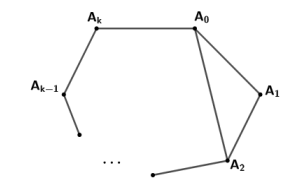
\includegraphics[scale=0.90]{Listas/lista1-ex11.png}
    \caption{Polígono de $k+1$ lados}
    \label{figur}
\end{figure}

O polígono $A_{0}A_{2} \cdots A_{k}$  que se obtém traçando o segmento $\overline{A_{0}A_{2}}$ tem $k$ lados. Consequentemente a soma dos seus ângulos internos é $S_{k}= \left( k-2 \right) \cdot180 ^{\circ}$. Agora, a soma dos ângulos internos do polígono original será a soma dos ângulos do triângulo $A_{0}A_{1}A_{2}$ adicionada de  $S_{k}$, isto é, \[S_{k+1}=S_{k}+180^{\circ} = \left( k-2 \right) \cdot180 ^{\circ} +180 ^{\circ} = \left( k+1-2 \right)\cdot180^{\circ}.\]

Assim, a soma dos ângulos internos de um polígono regular de $n$ lados de fato é $(n-2) \cdot 18^{\circ}.$

\end{solution}
\begin{exercicio}
Sabe-se que a forma trigonométrica do número complexo $z = a + bi$ é dada por
\[
z = \rho (\cos \theta + i \sen \theta),
\]
onde $\theta = \text{arg } z$ e $\rho = \abs{z} = \sqrt{a^2 + b^2}.$ Prove, utilizando o Princípio de Indução Finita, a fórmula de De Moivre, isto é, se $z = \rho (\cos \theta + i \sen \theta)$, então
\[
z^n = \rho^n (\cos (n\theta) + i \sen (n\theta)), \quad \forall n \in \mathbb{N}.
\]
\end{exercicio}

\begin{solution}
Comecemos com o caso \textbf{base}. Nessa situação, o caso base é dado para $n = 0,$ onde temos:
$$z^{0}= \rho ^{0} \left( \cos  \left( 0 \theta  \right) +i\cdot\sen  \left( 0 \theta  \right)  \right) = 1 \cdot \left( \cos (0) +i\cdot \sen \left( 0  \right) \right) =1 = z^{0}$$

Agora, suponha por \textbf{hipótese} que a fórmula de De Moivre é válida para um certo $n = k > 0,$ ou seja, 
$$z^{k}= \rho ^{k} \left( \cos  \left( k \theta  \right) +i\cdot\sen  \left( k \theta  \right)  \right)$$

Temos então que, para $n = k + 1,$
\begin{align*}z^{k+1}=\textcolor{RawSienna}{z^{k}}\cdot z^{1} &= \textcolor{RawSienna}{\left(  \rho ^{k} \left( \cos  \left( k \theta  \right) +i\cdot\sen  \left( k \theta  \right)  \right)  \right)}\cdot \left(  \rho  \left( \cos  \theta +i\cdot \sen  \theta  \right)  \right) \\&= \rho ^{k+1} \left( \cos  \left( k \theta  \right) +i\cdot\sen  \left( k \theta  \right)  \right) \cdot   \left( \cos  \theta +i\cdot \sen  \theta  \right)  \\&=
\rho ^{k+1} \left( \textcolor{Cerulean}{\cos  \left( k \theta  \right) \cos  \theta -\sen  \theta \sen  \left( k \theta  \right) }+i\cdot \left( \textcolor{Floresta}{\cos k \theta \sen  \theta +\sen k \theta \cos  \theta } \right)  \right) \\&=
\rho ^{k+1} \left( \textcolor{Cerulean}{\cos  \left( k \theta + \theta \right) }+i\cdot \left( \textcolor{Floresta}{\sen (k \theta + \theta) } \right)  \right) \\&=\rho ^{k+1} \left( \cos  \left(  \left( k+1 \right)  \theta  \right) +i\cdot\sen  \left(  \left( k+1 \right)  \theta  \right)  \right)
\end{align*}

Portanto, o \textbf{passo indutivo} está finalizado e a fórmula de De Moivre provada. 
\end{solution}


\begin{exercicio}
Seja $a \neq 0 \in \mathbb{Z}$ e $m \in \mathbb{N}.$ Definimos a potência não-negativa de $a$ do seguinte modo:
\[
a^m = \begin{cases}
1, & \mbox{se } m = 0\\
a, & \mbox{se } m = 1\\
a^{m-1} \cdot a, & \mbox{se } m > 1
\end{cases}.
\]
Prove que
\itens{
\task[\alt{a}] $a^m \cdot a^n = a^m+n, \forall m,n \in \mathbb{N};$
\task[\alt{b}] $(a^m)^n = a^{m \cdot n}, \forall m,n \in \mathbb{N}.$
}
\end{exercicio}

\begin{solution}
Provemos ambos os itens por indução:
\itens{
\task[\alt{a}] O caso base é $n = 0:$
$$a^{m}\cdot a^{0}\stackrel{def}{=}a^{m}\cdot 1=a^{m+0}=a^{m}$$
A hipótese de indução é que, para certo $n = k,$ é válido
$$a^{m}\cdot a^{k}=a^{m+k};k \in \Z.$$
Provemos agora que a afirmação é válida para $n = k +1:$
$$a^{m}\cdot a^{k+1}=a^{m}\cdot \left( a^{k}\cdot a^{1} \right) = \textcolor{Cyan}{\left( a^{m}\cdot a^{k} \right)}\cdot a^{1}=\textcolor{Cyan}{a^{m+k}}\cdot a^{1}\stackrel{def}{=}a^{m+k+1}$$
\task[\alt{b}] O caso base é $n = 0:$
$$\left( a^{m} \right) ^{0}\stackrel{def}{=}1=a^{m\cdot0}=a^{0}$$
A hipótese de indução é que, para certo $n = k,$ é válido
$$\left( a^{m} \right)^{k}=a^{m\cdot k};k \in \Z$$
Provemos agora que a afirmação é válida para $n = k +1:$
$$\left( a^{m} \right)^{k+1}= \textcolor{Green}{\left( a^{m} \right)^{k}}\cdot \left( a^{m} \right)^{1}=\textcolor{Green}{a^{m\cdot k}}\cdot a^{m}=a^{m\cdot k+m}=a^{m \left( k+1 \right)}$$
}
\end{solution}

\begin{exercicio}
Prove que $x - y$ divide $x^n - y^n$ para quaisquer inteiros $x,y$ distintos e $n \ge 1.$
\end{exercicio}
\begin{solution}
Vamos provar o resultado por indução. Primeiramente, observemos o \textbf{caso base} $n=1:$
$$x^{1}-y^{1}=x-y=1\cdot\left( x-y \right)$$
Como \textbf{hipótese de indução}, assuma que $x - y$ divide $x^n - y^n$ para $n=k>1,$ ou seja, que
$$x^{k}-y^{k}=t \left( x-y \right) ;t \in \Z $$
Realizemos agora o \textbf{passo indutivo}, mostrando que a afirmação é válida para $n=k+1$:
\begin{align*}
x^{k+1}-y^{k+1}&=x\cdot x^{k}-y\cdot y^{k}\\
&=x\cdot x^{k}\textcolor{Plum}{-x\cdot y^{k}+x\cdot y^{k}}-y\cdot y^{k}\\
&=x \textcolor{PineGreen}{\left( x^{k}-y^{k} \right)} +y^{k} \left( x-y \right)\\
&=x\cdot \textcolor{PineGreen}{t \left( x-y \right)} +y^{k} \left( x-y \right)\\
&=\left( x-y \right)  \textcolor{RawSienna}{\left( xt+y^{k} \right)}\\ 
&= \left( x-y \right) \textcolor{RawSienna}{q}; \quad q \in \Z
\end{align*}
\end{solution}
%\newpage%parasolucoes
\begin{exercicio}
Para todo inteiro $n \ge 1,$ prove que
\itens{
\task[\alt{a}] $\dfrac{1}{1 - x} = 1 + x + x^2 + \ldots + x^{n-1} + \dfrac{x^n}{1-x};$
\task[\alt{b}] $1 + 2 + 2^2 + \ldots + 2^{n-1} = 2^n - 1$ (\textsf{[Dica:]} Use o item anterior).
}
\end{exercicio}
\begin{solution}
\itens{
\task[\alt{a}] O caso base é $n = 1.$ Temos:

$$1+\frac{x}{1-x}=\frac{1-x+x}{1-x}=\frac{1}{1-x}$$
Agora, assuma por hipótese que a afirmação é válida para $n=k>1,$ ou seja, 
$$1+x+ \cdots +x^{k-1}+\frac{x^{k}}{1-x}=\frac{1}{1-x}$$

Vamos provar que o resultado é válido para $n = k + 1.$ Para isso, observe primeiramente que, da hipótese de indução, temos
$$1+x+ \cdots +x^{k-1}+\frac{x^{k}}{1-x}=\frac{1}{1-x} \Rightarrow$$
$$1+x+ \cdots +x^{k-1}=\frac{1}{1-x}-\frac{x^{k}}{1-x}$$
Utilizando isso, estamos aptos a realizar o passo indutivo para provar que
$$1+x+ \cdots +x^{k-1}+x^k+\frac{x^{k+1}}{1-x}=\frac{1}{1-x}.$$
De fato,
\begin{align*}
\textcolor{Cyan}{1+x+ \cdots +x^{k-1}}+x^{k}+\frac{x^{k+1}}{1-x}&=\textcolor{Cyan}{\frac{1}{1-x}-\frac{x^{k}}{1-x}}+x^{k}+\frac{x^{k+1}}{1-x}\\&
=\frac{1-x^{k}+x^{k} \left( 1-x \right) +x^{k+1}}{1-x}\\&
=\frac{1-x^{k}+x^{k} - x^{k+1} +x^{k+1}}{1-x}\\
&=\frac{1}{1-x}.
\end{align*}
\task[\alt{b}] Para $x=2$, temos:
$$1+2+2^{2}+ \cdots +2^{n-1}=\frac{1}{1-2}-\frac{2^{n}}{1-2}=-1-\frac{2^{n}}{-1}=2^{n}-1$$
}
\end{solution}

\begin{exercicio}\textcolor{Blue}{*}
Seja $n$ um inteiro positivo. Mostre que
\itensladoalado{2}{
\task[\alt{a}] $\sum\limits_{k=0}^n  (-1)^k \binom{n}{k} = 0;$
\task[\alt{b}]
$\sum\limits_{k=0}^n \binom{n}{k}^2 = \binom{2n}{n}$
}
\end{exercicio}
\begin{solution}
\itens{
\task[\alt{a}] Para resolver esse item, vamos considerar a expansão de $(x + y)^n:$

\begin{align}\label{binnew}
\left( x+y \right) ^{n}= \binom{n}{0} x^{n}y^{0}+ \binom{n}{1}x^{n-1}y^{1}+ \cdots + \binom{n}{n-1}x^{1}y^{n-1}+ \binom{n}{n} x^{0}y^{n}
\end{align}

Como a soma se trata de termos alternantes, ou seja,
\[
\sum\limits_{k=0}^n  (-1)^k \binom{n}{k} = \binom{n}{0} - \binom{n}{1} + \binom{n}{2} -  \ldots + (-1)^{n-1} \binom{n}{n-1} + (-1)^{n} \binom{n}{n},
\]
Podemos colocar $x=1$ e $y=-1$ na Equação (\ref{binnew}) para obter a soma acima, chegando assim a:
\begin{align*}
\left( 1+(-1) \right) ^{n}&= \binom{n}{0}1^{n} \left( -1 \right) ^{0}+ \binom{n}{1} 1^{n-1} \left( -1 \right) ^{1}+ \cdots + \binom{n}{n-1} 1^{1} \left( -1 \right) ^{n-1}+ \binom{n}{n} 1^{0} \left( -1 \right) ^{n}\\
0^{n}&= \binom{n}{0}\left( -1 \right) ^{0}+ \binom{n}{1}\left( -1 \right) ^{1}+ \cdots + \binom{n}{n-1}\left( -1 \right) ^{n-1}+ \binom{n}{n}\left( -1 \right) ^{n}\\
0&= \binom{n}{0}\left( -1 \right) - \binom{n}{1} + \cdots + \binom{n}{n-1}\left( -1 \right) ^{n-1}+ \binom{n}{n}\left( -1 \right) ^{n}\\
0&= \sum _{k=0}^{n} \left( -1 \right) ^{k} \binom{n}{k}
\end{align*}
}
\itens{
\task[\alt{b}] Como nos coeficientes binomiais temos a presença do termo $2n,$ vamos analisar o comportamento de
$$\left( x+1 \right) ^{2n}= \left( x+1 \right) ^{n} \left( 1+x \right) ^{n}.$$
}
Desenvolvendo cada binômio separadamente, temos:
\begin{align*}
\left( 1+x \right) ^{2n}&= \binom{2n}{0} x^{2n}+ \binom{2n}{1}x^{2n-1}+ \cdots + \binom{2n}{n}x^{n}+ \cdots + \binom{2n}{2n-1}x^{1}+ \binom{2n}{2n}x^{0}\\
\left( x+1 \right) ^{n}&= \binom{n}{0}x^{n}+ \binom{n}{1}x^{n-1}+ \cdots + \binom{n}{n-1}x^{1}+ \binom{n}{n}x^{0}\\
\left( 1+x \right) ^{n}&= \binom{n}{0}x^{0}+ \binom{n}{1}x^{1}+ \cdots + \binom{n}{n-1}x^{n-1}+ \binom{n}{n}x^{n}
\end{align*}

Ao multiplicarmos os dois últimos, obtemos um polinômio equivalente ao primeiro, ou seja:
$$\binom{2n}{0}x^{2n}+ \binom{2n}{1} x^{2n-1}+ \cdots + \binom{2n}{n}x^{n}+ \cdots + \binom{2n}{2n-1}x^{1}+ \binom{2n}{2n}x^{0} =$$
$$\left[ \binom{n}{n}\cdot \binom{n}{0}  \right] x^{0}+ \cdots +\left[  \binom{n}{0} ^{2}+ \binom{n}{1}^{2}+ \cdots + \binom{n}{n}^{2} \right]x^{n}+ \cdots +  \left[  \binom{n}{0}\cdot \binom{n}{n} \right]x^{2n}$$

Note que o coeficiente de $x^{n}$ nos dois polinômios devem ser iguais. Assim:

$$ \left[  \binom{n}{0}^{2}+ \binom{n}{1}^{2}+ \cdots + \binom{n}{n}^{2} \right] = \binom{2n}{n} \Rightarrow$$

$$\sum_{k=0}^{n} \binom{n}{k}^{2}= \binom{2n}{n}$$


\end{solution}

\begin{exercicio}
Prove por indução finita para todo $n > 1$ que
\itens{
\task[\alt{a}] $\dfrac{1}{n+1} + \dfrac{1}{n+2} + \cdots + \dfrac{1}{2n} > \dfrac{13}{24};$
\task[\alt{b}] $\left(1 - \dfrac{1}{4} \right) \cdot \left( 1 - \dfrac{1}{9} \right) \cdot \ldots \cdot \left( 1 - \dfrac{1}{n^2} \right) = \dfrac{n+1}{2n};$
\task[\alt{c}] $1 \cdot 1! + 2 \cdot 2! + \ldots + n \cdot n! = (n+1)! - 1,$
\task[\alt{d}] $\dfrac{1}{1 \cdot 2} + \dfrac{1}{2 \cdot 3} + \ldots + \dfrac{1}{n \cdot (n + 1)} = \dfrac{n}{n+1}.$
}
\end{exercicio}
\begin{solution}
\itens{
\task[\alt{a}] \textbf{Caso :} $n = 2.$ Para $n = 2,$ temos que
$$\frac{1}{3}+\frac{1}{4}=\frac{14}{24}>\frac{13}{24}$$
\textit{Hipótese}: \textbf{Hipótese:} Suponha que, para $n=k>2,$
$$\frac{1}{k+1}+\frac{1}{k+2}+ \cdots +\frac{1}{2k}>\frac{13}{24}$$
\textit{Passo Indutivo}: Para $n=k+1,$ temos
\begin{align*}
\frac{1}{(k+1)+1} + \ldots + \frac{1}{2(k+1)}&=
\frac{1}{k+2}+\frac{1}{k+3}+\cdots+\frac{1}{2k}+\frac{1}{2k+1}+\frac{1}{2k+2}\\&=  \textcolor{Magenta}{\frac{1}{k+1} + \frac{1}{k+2}+\cdots+\frac{1}{2k}}+\frac{1}{2k+1}+\frac{1}{2k+2} - \frac{1}{k+1}\\&>\textcolor{Magenta}{\frac{13}{24}}+\frac{1}{2k+1}+\frac{1}{2k+2}-\frac{1}{k+1}\\&=
\frac{13}{24}+\frac{1}{2k+1}-\frac{1}{2k+2}\\&>\frac{13}{24}+\frac{1}{2k+2}-\frac{1}{2k+2}=\frac{13}{24}.
\end{align*}
\task[\alt{b}] \textbf{Caso base:} O caso base é $n = 2.$ Temos
$$\left( 1-\frac{1}{4} \right) =\frac{3}{4}=\frac{2+1}{2\cdot2}$$
\textit{Hipótese}: Suponha que, para $n=k>2,$
$$\left( 1-\frac{1}{4} \right)\cdot \left( 1-\frac{1}{9} \right)  \cdots  \left( 1-\frac{1}{k^{2}} \right) =\frac{k+1}{2k}$$
\textit{Passo Indutivo}: Provemos que a afirmação é válida para $n=k+1:$
\begin{align*}\textcolor{Magenta}{\left( 1-\frac{1}{4} \right)\cdot \left( 1-\frac{1}{9} \right)  \cdots  \left( 1-\frac{1}{k^{2}} \right)} \cdot \left( 1-\frac{1}{ \left( k+1 \right) ^{2}} \right)&=
\textcolor{Magenta}{\frac{k+1}{2k}}\cdot \left( 1-\frac{1}{ \left( k+1 \right) ^{2}} \right) \\&=\frac{k+1}{2k}\cdot \left( \frac{ \left( k+1 \right) ^{2}-1}{ \left( k+1 \right) ^{2}} \right) \\&=\frac{k+1}{2k}\cdot \left( \frac{k^{2}+2k}{ \left( k+1 \right) ^{2}} \right)\\& =\frac{ \left( k+2 \right) }{2 \left( k+1 \right) }\\& =\frac{ \left( k+1 \right)+1 }{2 \left( k+1 \right) }.
\end{align*}
\task[\alt{c}] \textbf{Caso base}: $n=1$
$$1\cdot1!=1 \quad \mbox{e} \quad \left( 1+1 \right)!-1=2!-1=2-1=1$$
\textit{Hipótese}: Suponha a afirmação válida para $n=k>1,$ ou seja,
$$1\cdot1!+2\cdot2!+ \cdots +k\cdot k!= \left( k+1 \right) !-1$$
\textit{Passo}: Vejamos que a afirmação é válida para $n=k+1:$
\begin{align*}
\textcolor{Magenta}{1\cdot1!+2\cdot2!+ \cdots +k\cdot k!}+ \left( k+1 \right)  \left( k+1 \right) !&= \textcolor{Magenta}{\left( k+1 \right) !-1}+ \left( k+1 \right)  \left( k+1 \right) ! \\&=
\textcolor{Cyan}{\left( k+1 \right) !} \left( 1+(k+1) \right) -1\\&= \left( k+2 \right)  \left( k+1 \right) !-1= \textcolor{Cyan}{\left( k+2 \right) !}-1.
\end{align*}
\task[\alt{d}] \textit{Caso Base}: Para $n=1,$ temos
$$\frac{1}{1\cdot \left( 1+1 \right) }=\frac{1}{2}=\frac{1}{1+1}$$
\textit{Hipótese}: Suponha a validade para $n=k>1:$
$$\frac{1}{1\cdot2}+\frac{1}{2\cdot3}+ \cdots +\frac{1}{k \left( k+1 \right) }=\frac{k}{k+1}$$
\textit{Passo Indutivo}: Provemos que a afirmação é válida para $n=k+1:$
\begin{align*}
\textcolor{Magenta}{\frac{1}{1\cdot2}+\frac{1}{2\cdot3}+ \cdots +\frac{1}{k \left( k+1 \right) }}+\frac{1}{ \left( k+1 \right)  \left( k+2 \right) }&=\textcolor{Magenta}{\frac{k}{k+1}}+\frac{1}{ \left( k+1 \right)  \left( k+2 \right) }\\&=\frac{k \left( k+2 \right) +1}{ \left( k+1 \right)  \left( k+2 \right) }\\&=
\frac{ \left( k^{2}+2k+1 \right) }{ \left( k+1 \right)  \left( k+2 \right) }\\&=\frac{ \left( k+1 \right) ^{2}}{ \left( k+1 \right)  \left( k+2 \right) }=\frac{k+1}{k+2}.
\end{align*}


}
\end{solution}


\begin{exercicio}
\itens{
\task[\alt{a}] Considere a sequência de números inteiros $(a_n)_{n \ge 0}$ dada por
\[
a_n = \begin{cases}
2, & \mbox{se } n = 0;\\
3, & \mbox{se } n = 1;\\
3a_{n-1} - 2a_{n-2}, & \mbox{se } n \ge 2
\end{cases}.\]

Mostre que 
\[
a_n = 2^n + 1, \quad \forall n \ge 0.
\]

\task[\alt{b}] Considere a sequência de números inteiros $(b_n)_{n \ge 0}$ dada por
\[
b_n = \begin{cases}
0, & \mbox{se } n = 0;\\
1, & \mbox{se } n = 1;\\
3b_{n-} - 2b_{n-2}, & \mbox{se } n \ge 2
\end{cases}.\]
Mostre que 
\[
b_n = 2^n - 1, \quad \forall n \ge 0.
\]
\task[\alt{c}] Considere a \textit{Sequência de Fibonacci} $(F_n)_{n \ge 0}$ dada por
\[
F_n = \begin{cases}
0, & \mbox{se } n = 0;\\
1, & \mbox{se } n = 1;\\
F_{n-1} + F_{n-2}, & \mbox{se } n \ge 2
\end{cases}.\]
Mostre que 
\itens{
\task[\alt{i}] $F_n^2 - F_{n+1}F_{n-1} = (-1)^{n+1};$
\task[\alt{ii}] $F_{n+1}F_{n+2} - F_{n}F_{n+3} = (-1)^n.$
}
}
\end{exercicio}
\begin{solution}
Vamos utilizar a segunda forma do Princípio da Indução Finita:
\itens{
\task[\alt{a}] \textbf{Caso Base}: Vejamos que a afirmação é válida para $n = 0$ e $n = 1:$
}
$n=0$: $$2^{0}+1=2=a_{0}$$
$n=1$: $$2^{1}+1=3=a_{1}$$
\textbf{Hipótese}: Suponha que a afirmação é válida \textbf{para todo} $n \geq k \geq 1,$ ou seja, para $k$ entre $1$ e $n,$ inclusive, temos
$$a_{k}=2^{k}+1$$
\textbf{Passo Indutivo}: Provemos que a afirmação é válida para $n=k+1:$
\begin{align*}
    a_{k+1}=3\textcolor{RawSienna}{a_{k}}-2 \textcolor{PineGreen}{a_{k-1}}&=3 \textcolor{RawSienna}{\left( 2^{k}+1 \right)} -2 \textcolor{PineGreen}{\left( 2^{k-1}+1 \right)}\\ &=3\cdot 2^{k}+3-2^{k}-2\\ &=
2\cdot2^{k}+1\\ &=2^{k+1}+1.
\end{align*}
\itens{
\task[\alt{b}] \textbf{Caso Base}: Vejamos que a afirmação é válida para $n = 0$ e $n = 1:$}
$n=0$: $$2^{0}-1=0=b_{0}$$
$n=1$: $$2^{1}-1=1=b_{1}$$
\textbf{Hipótese}: Suponha que a afirmação é válida \textbf{para todo} $n \geq k \geq 1,$ ou seja, para $k$ entre $1$ e $n,$
$$b_{k}=2^{k}-1$$
\textit{Passo Indutivo}: Provemos que a afirmação é válida para $n=k+1:$
\begin{align*}
b_{k+1}=3\textcolor{RawSienna}{b_{k}}-2\textcolor{PineGreen}{b_{k-1}}&=3 \textcolor{RawSienna}{\left( 2^{k}-1 \right)} -2 \textcolor{PineGreen}{\left( 2^{k-1}-1 \right)} \\&=3\cdot2^{k}-3-2^{k}+2\\&=
2\cdot2^{k}-1=2^{k+1}-1.
\end{align*}
\itens{
\task[\alt{c}] Observe que}
$$F_{2}=F_{1}+F_{0}=1+0=1$$
$$F_{3}=F_{2}+F_{1}=1+1=2$$
$$F_{4}=F_{3}+F_{2}=2+1=3$$
$$F_{5}=F_{4}+F_{3}=3+2=5$$
Vamos provar ambos os itens por indução:
\itens{
\task[\alt{i}] \textbf{Caso base:} Para $n = 2,$ temos 
 $$F_{2}^{2}-F_{3}F_{1}=1^{2}-2\cdot1=-1= \left( -1 \right) ^{2+1}$$
 
 \textbf{Hipótese:} Suponha que a afirmação é válida \textbf{para todo} $n \geq k \geq 1,$ ou seja, para $k$ entre $1$ e $n,$
 $$F_{k}^{2}-F_{k+1}F_{k-1}= \left( -1 \right) ^{k+1}$$
 
 \textbf{Passo indutivo:} Para $n = k+1,$
 \begin{align*}
F_{k+1}^{2}-\textcolor{NavyBlue}{F_{k+2}}F_{k}&=F_{k+1}^{2}- \textcolor{NavyBlue}{\left( F_{k+1}+F_{k} \right)} F_{k}\\&=F_{k+1}^{2}-F_{k}\cdot F_{k+1}-F_{k}^{2}\\&=
F_{k+1} \textcolor{Plum}{\left( F_{k+1}-F_{k} \right)} -F_{k}^{2}\\&= F_{k+1}\textcolor{Plum}{F_{k-1}}-F_{k}^{2}\\&=
- \textcolor{RawSienna}{\left( F_{k}^{2}-F_{k+1}F_{k-1} \right)} \\&=-\textcolor{RawSienna}{ \left( -1 \right) ^{k+1}}= \left( -1 \right) ^{k+2}.
\end{align*}
\task[\alt{ii}] \textbf{Caso base:} Para $n = 2,$ temos 
 $$F_{2}^{2}-F_{3}F_{1}=1^{2}-2\cdot1=-1= \left( -1 \right) ^{2+1}$$
 
 \textbf{Hipótese:} Suponha que a afirmação é válida \textbf{para todo} $n \geq k \geq 1,$ ou seja, para $k$ entre $1$ e $n,$
$$F_{3}F_{4}-F_{2}F_{5}=2\cdot3-1\cdot5=1= \left( -1 \right) ^{2}$$
 
 \textbf{Passo indutivo:} Para $n = k+1,$
\begin{align*}
\textcolor{NavyBlue}{F_{k+2}}F_{k+3}-F_{k+1}\textcolor{Plum}{F_{k+4}}&=\textcolor{NavyBlue}{\left( F_{k}+F_{k+1} \right)} F_{k+3}-F_{k+1} \textcolor{Plum}{\left( F_{k+2}+F_{k+3} \right)}\\ 
&=F_{k}F_{k+3}+\cancel{F_{k+1}F_{k+3}}-F_{k+1} F_{k+2}-\cancel{F_{k+1}F_{k+3}}\\
&=F_{k}F_{k+3}-F_{k+1} F_{k+2}\\
&=-\textcolor{RawSienna}{(F_{k+1} F_{k+2}-F_{k}F_{k+3})}\\
&=-\textcolor{RawSienna}{(-1)^{k}}=(-1)^{k+1}.
\end{align*}
}

\end{solution}

\begin{exercicio}
Prove que, se $n$ é um múltiplo de $8$, então $F_{n}$ é múltiplo de $7.$

\textsf{[Dica:]} Prove que $F_{n+8} = 7F_{n+4} - F_n.$
\end{exercicio}
\begin{solution}
Vamos provar inicialmente que $F_{n + 8} = 7F_{n+4} - F_n.$

Faremos a demonstração por indução:

\textbf{Caso Base:} Para $n = 0,$ temos
\[
F_{0 + 8} = F_8 = 21 = 7 \cdot 3 - 0 = 7 F_{0 + 4} - F_0
\]
Para $n = 1,$ temos
\[
F_{1 + 8} = F_9 = 34 = 7 \cdot 5 - 1 = 7 F_{1 + 4} - F_1
\]

\textbf{Hipótese:} Suponha que a afirmação é válida para todo $n$ com $0 \le n \le k,$ ou seja,
$F{k + 8} = 7F_{k+4} - F_k.$

\textbf{Passo indutivo:} Vamos provar que o resultado é válido para $n = k+1:$
\begin{align*}
F_{(k+1)+8} &= F_{k+9} \\&= \textcolor{RawSienna}{F_{k+8}} + \textcolor{Magenta}{F_{k+7}} \\&= \textcolor{RawSienna}{7F_{k+4} - F_k} + \textcolor{Magenta}{7F_{k + 3} - F_{k-1}} \\&= 7(F_{k+4} + F_{k+3} - (F_{k} + F_{k-1}) \\&= 7F_{k+5} - F_{k+1} 
\end{align*}

Vejamos agora que $F_n$ é múltiplo de $7.$ se $n$ é múltiplo de $8.$ Sendo $n$ múltiplo de $8$, podemos escrevê-lo na forma $n = 8t,$ onde $t \in \mathbb{N}.$ Vamos mostrar esse resultado por indução em $t.$

\textbf{Caso Base:} Para $t = 0,$ temos
\[
F_{8 \cdot 0} = F_0 = 0 = 0 \cdot 7.
\]

\textbf{Hipótese:} Suponha que, para $t = k,$ é válido que
\[
F_{8k} = 7 q, \quad q \in \mathbb{N}.
\]

\textbf{Passo Indutivo:} Vamos verificar que, para $t = k +1,$ $F_{8(k+1)}$ é múltiplo de $7.$ Com auxílio do fato demonstrado acima, temos
\begin{align*}
  F_{8(k+1)} &= F_{8k + 8} \\&= 7F_{8k+4} - \textcolor{Magenta}{F_{8k}} \\&= 7F_{8k+4} - \textcolor{Magenta}{7q} \\&= 7\textcolor{RawSienna}{(F_{8k+4} - q)} \\&= 7 \textcolor{RawSienna}{r}, r \in \mathbb{N}.
\end{align*}
\end{solution}

\begin{exercicio}\textcolor{Blue}{*}
Prove que todo número natural pode ser representado como uma soma de diversos números de Fibonacci distintos.
\end{exercicio}
\begin{solution}
Provaremos o resultado por indução em $n,$ pela segunda forma. Comecemos com o \textbf{caso base}. Se $n = 0, n = 1$ ou $n = 2,$ então a existência da representação desejada é trivial.

Agora vamos supor por \textbf{hipótese} que todo número natural menor que $n$ pode ser representado como uma soma de diversos números de Fibonacci distintos. Agora, vamos encontrar o maior número de Fibonacci menor ou igual a $n.$ Suponha que é $F_m;$ ou seja, $F_m \le n < F_{m+1}.$ A diferença $d = n - F_m$ é menor do que $n$ e também menor do que $F_m,$ já que $F_{m+1} = F_{m} + F_{m-1}.$ Pela hipótese de indução, $d$ pode ser representado como uma soma de diversos números de Fibonacci distintos e é claro que $F_m$ é grande demais para ser incluído. Logo, somando $F_m,$ obtemos a expressão desejada para $n,$ já que $d$ pode ser escrito como soma de números de Fibonacci distintos, e
\[n = d + F_m.\]
\end{solution}


\begin{exercicio}
 O que há de errado com a seguinte demonstração por indução de que para todo inteiro positivo $n$ nós temos $a^{n-1} = 1?$
 \begin{quote}
     Demonstração: Para $n = 1, a^{1-1} = a^0 = 1,$ correto. Assumindo o teorema válido para $k \le n,$ temos para $n + 1:$
     \[
     a^{(n+1)-1} = a^n = \dfrac{a^{n-1} \cdot a^{n-1}}{a^{n-2}} = \dfrac{1 \cdot 1}{1} = 1,
     \]como desejávamos.
 \end{quote}
\end{exercicio}
\begin{solution}
Vamos observar como o passo indutivo foi desenvolvido. 
     \[
     a^{(n+1)-1} = a^n = \textcolor{Red}{\dfrac{a^{n-1} \cdot a^{n-1}}{a^{n-2}}} = \dfrac{1 \cdot 1}{1} = 1,
     \]
Atente para o fato de que, na expressão em \textcolor{Red}{vermelho}, o autor da demonstração utilizou que $a^{n-1} = 1$ \textbf{e} $a^{n-2} = 1,$ o que não foi provada, já que em seu caso base, apenas mostrou-se a validade da expressão para $n = 1,$ e não para $n = 2,$ o qual claramente a afirmação está equivocada, visto que $a^{2-1} = a^1 = a \neq 0.$ Assim, houve uma confusão entre o uso da primeira e da segunda forma do Princípio da Indução Finita, advindo daí o erro da demonstração em questão.

\end{solution}

\begin{exercicio}\textcolor{Blue}{*}
É dado um conjunto de $n$ pontos em um círculo e cada par de pontos está ligado por um segmento. Acontece que três desses segmentos nunca se encontram no mesmo ponto. Em quantas partes eles dividem o interior do círculo?
\end{exercicio}
\begin{solution}
Vamos primeiramente iniciar uma busca para a fórmula que registre o número $\mathcal{P}(n)$ de partes nas quais o círculo é dividido. Para $n = 1, 2,$ é óbvio que $\mathcal{P}(1) = 1,$ $\mathcal{P}(2) = 2.$ 

Fazendo os desenhos para $n = 3, 4$ e $5,$ obtemos que $\mathcal{P}(3) = 4, \mathcal{P}(4) = 8$ e $\mathcal{P}(5) = 16,$ como mostrado na figura abaixo:
\newpage
%https://oeis.org/A000127/a000127.jpg
\begin{figure}[!htb]
    \centering
    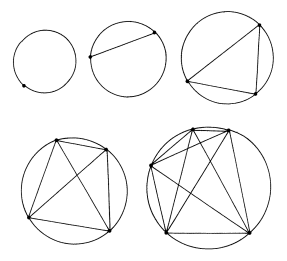
\includegraphics[scale=1.25]{Listas/lista_1ex18.png}
    \caption{Desenhos para $\mathcal{P}(1), \mathcal{P}(2), \mathcal{P}(3), \mathcal{P}(4)$ e $\mathcal{P}(5).$}
    \label{figuraa}
\end{figure}
Poderíamos baseado nessas observações conjecturar que $\mathcal{P}(n) = 2^{n-1},$ mas veremos que isso não ocorre. 

Se o círculo possui $n$ pontos, então existem $\binom{n}{4}$ intersecções de cordas dentro do círculo, pois cada conjunto de quatro pontos fornece apenas uma dessas intersecções. Assim, o número de vértices na figura deve ser $V = n + \binom{n}{4}.$ Para encontrar o número de arestas, contemos suas extremidades. Existem $n+1$ delas em cada um dos $n$ pontos e quatro em cada uma das $\binom{n}{4}$ intersecções, ou seja,
\[
2A = n(n+1) + 4 \binom{n}{4}. 
\]
Pela Fórmula de Euler $V - A + F = 1,$ o número de regiões dentro do círculo deve ser
\begin{align*}
    F = 1 + \textcolor{Blue}{A} - \textcolor{PineGreen}{V} &= 1 + \textcolor{Blue}{\frac{n(n+1)}{2} + 2 \binom{n}{4}} - \left(\textcolor{PineGreen}{ n + \binom{n}{4}}\right) 
    \\&= \binom{n}{4} + \frac{n(n+1) -2n}{2} + 1
    \\&= \binom{n}{4} + \frac{n(n-1)}{2} + 1
    \\&= \binom{n}{4} + \binom{n}{2} + 1
\end{align*}
Vamos provar então que 
\[
\mathcal{P}(n) = \binom{n}{4} + \binom{n}{2} + 1.
\]
Para o nosso \textbf{caso base}, vamos considerar.

Para o \textbf{passo indutivo}, suponha que para algum $n = k,$ temos que
\[
\mathcal{P}(k) = \binom{k}{4} + \binom{k}{2} + 1.
\]
Vamos mostrar que a fórmula é válida para $\mathcal{P}(k+1).$

Para isso, observe que, partindo do círculo com as $\mathcal{P}(k)$ marcadas, ao adicionar um novo ponto, ligando aos demais $k$ pontos, teremos a formação de $k$ novas regiões. Além disso, como três segmentos não podem se encontrar no mesmo ponto, teremos outras $\binom{k}{3}$ regiões formadas. Assim:
\begin{align*}
    \mathcal{P}(k+1) &= \textcolor{RawSienna}{\mathcal{P}(k)} + \dbinom{k}{3} + \textcolor{Magenta}{k}
    \\&= \textcolor{RawSienna}{\dbinom{k}{4} + \dbinom{k}{2} + 1} + \dbinom{k}{3} + \textcolor{Magenta}{\dbinom{k}{1}}
    \\&= \textcolor{JungleGreen}{\dbinom{k}{4} + \dbinom{k}{3}} + \textcolor{Plum}{\dbinom{k}{2} + \dbinom{k}{1}} + 1 
    \\&= \textcolor{JungleGreen}{\dbinom{k+1}{4}} + \textcolor{Plum}{\dbinom{k+1}{2}} + 1,
\end{align*}
onde no último passo utilizamos a Relação de Stifel:
\[
\dbinom{n}{p-1} + \dbinom{n}{p} = \dbinom{n+1}{p}
\]
Assim, mostramos que $\mathcal{P}(k+1) = \dbinom{k+1}{4} + \dbinom{k+1}{2} + 1.$

Uma curiosidade é que, $\mathcal{P}(10) = 256,$ como mostrado na figura abaixo:
\begin{figure}[!htb]
    \centering
    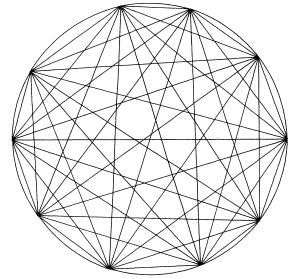
\includegraphics[scale=0.90]{Listas/lista_1ex182.png}
    \label{figuraa}
\end{figure}
\end{solution}

\begin{exercicio}\textcolor{Blue}{*} \textsf{[Pizza de Steiner]}
Qual é o maior número de partes em que se pode dividir o plano com $n$ cortes retos?
\end{exercicio}
\begin{solution}
Denotando o número máximo de pedaços com $n$ cortes por $p_n,$
vamos provar por indução a fórmula:
\[
p_n = \dfrac{n(n+1)}{2} + 1.
\]
No \textbf{caso base}, para $n = 1,$ ou seja, com apenas um corte, é claro que só podemos
obter dois pedaços. Portanto, a fórmula está correta, pois
\[
p_1 = \dfrac{1(1+1)}{2} + 1 = 2.
\]
Admitamos agora como \textbf{hipótese} que, para algum $n= k$, a fórmula para $p_k$ esteja correta. Vamos mostrar que a fórmula para $p_{k+1}$ também está correta.

Suponhamos que, com $k$ cortes, obtivemos o número máximo
$\frac{k(k + 1)}{2} + 1$ de pedaços e queremos fazer mais um corte, de modo a obter o maior número possível de pedaços. Vamos conseguir isso se o $(k + 1)$-ésimo corte encontrar cada um dos $k$ cortes anteriores em pontos que não são de interseção de dois cortes. 

Por outro lado, se o $(k+ 1)$-ésimo corte encontra todos os $k$ cortes anteriores, ele produz $k + 1$ novos pedaços: o corte começa em um determinado pedaço e, ao encontrar o primeiro corte, ele separa em dois o pedaço em que está, entrando em outro pedaço. Ao encontrar o segundo corte, ele separa em dois o pedaço em que está, entrando em outro pedaço, e assim sucessivamente, até encontrar o $k$-ésimo corte separando o último pedaço em que entrar em dois. Assim, são obtidos $k + 1$ pedaços a mais dos que já existiam; logo,
\begin{align*}
    p_{k+1} &= \textcolor{Cyan}{p_k} + k + 1 \\&= \textcolor{Cyan}{\dfrac{n(n+1)}{2}+1} + n + 1 \\&= \dfrac{(n+1)(n+2)}{2} + 1,
\end{align*}
o que mostra que a fórmula está correta para $n + 1$ cortes.
\end{solution}

\begin{exercicio}
Suponha um campeonato de futebol com $n$ times onde todos jogam contra
todos uma única vez. Prove por indução que o número total de jogos é $\dfrac{n(n-1)}{2}.$
\end{exercicio}
\begin{solution}
Seja $\mathcal{J}(n)$ o total de jogos do campeonato de futebol com $n$ times onde todos jogam contra todos uma única vez. Vamos provar o resultado por indução em $n:$

\textbf{Caso base:} Para $n = 2,$ suponha que as equipes que disputem o torneio sejam A e B. Só haverá então $1$ jogo, justamente o confronto A x B, e portanto
\[
\mathcal{J}(2) = 1 = \dfrac{2(2-1)}{2}
\]

\textbf{Hipótese:} Suponha que para $n = k,$ o total de jogos de futebol do campeonato seja 
\[
\mathcal{J}(k) = \dfrac{k(k-1)}{2}.
\]
\textbf{Passo indutivo:} Provemos que $\mathcal{J}(k+1) = \dfrac{(k(k+1)}{2}.$ Para isso, considere que as equipes $A_1, A_2, \ldots,$ $A_k$ e $A_{k+1}$ disputaram o torneio. Pela hipótese de indução, um torneio com as $k$ equipes $A_1, A_2, \ldots, A_k$ terá exatamente $\mathcal{J}(k) = \dfrac{k(k-1)}{2}$ partidas disputadas. Para um torneio com a adição de $A_{k+1},$ este deverá disputar todos os confrontos $A_{k+1} \text{ x } A_1$, $A_{k+1} \text{ x } A_2$, ..., $A_{k+1} \text{ x } A_{k-1}$ e $A_{k+1} \text{ x } A_{k},$ fazendo um total de $k$ jogos. Logo, o total de partidas disputadas será
\begin{align*}
\mathcal{J}(k + 1) &= \textcolor{RawSienna}{\mathcal{J}(k)} + k
    \\&= \textcolor{RawSienna}{\dfrac{k(k-1)}{2}} + k \\&= \dfrac{k(k-1)}{2} + \dfrac{2k}{2} \\&= \dfrac{k(k-1) + 2k}{2} \\&= \dfrac{k^2 - k + 2k}{2} \\&= \dfrac{k^2 + k}{2} \\&= \dfrac{k(k+1)}{2}.
\end{align*}
\end{solution}

\begin{exercicio}\textcolor{Blue}{*}
Faça uma conjectura sobre as somas das diagonais ascendentes
no Triângulo de Pascal conforme indicado. Prove que sua conjectura é verdadeira.
\begin{figure}[ht]
    \centering
    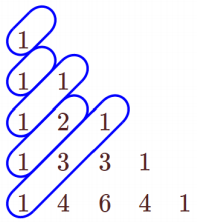
\includegraphics[scale=0.90]{Listas/lista1-ex21.png}
    \label{figur}
\end{figure}
\end{exercicio}

\begin{solution}
Temos então que provar que
\[
\sum\limits_{p = 0}^{n} \binom{n - p}{p} = \binom{n}{0} + \binom{n-1}{1} + \binom{n - 2}{2} + \ldots + \binom{0}{n} = F_{n+1}
\]
\textbf{Caso base:} Para $n = 0,$ temos
\[
\binom{0}{0} = 1 = F_{0+1}
\]

\textbf{Hipótese:} Suponha que o resultado é válido para $n = k,$ ou seja, 
\[
\sum\limits_{p = 0}^{k} \binom{k - p}{p} = F_{k+1}
\]
\textbf{Passo indutivo:} Vejamos a validade da identidade para $n = k + 1.$ Para isso, vamos utilizar a relação de Stifel:
$$
\binom{n}{k}=\binom{n-1}{k}+\binom{n-1}{k-1}
$$
Agora, temos que

\begin{align*}
  \sum\limits_{p = 0}^{k+1} \binom{(k+1) - p}{p} &=\binom{k+1}{0}+\sum_{p=1}^{k}\textcolor{PineGreen}{\binom{(k+1)-p}{p}}\\&=\binom{k}{0}+\sum_{p=1}^{k}\textcolor{PineGreen}{\left[\binom{k-p}{p}+\binom{k-p}{p-1}\right]}\\&=\textcolor{NavyBlue}{\binom{k}{0}+\sum\limits_{p=1}^{k}\binom{k-p}{p}}+\sum\limits_{p=1}^{k}\binom{k-p}{p-1} \\&=\textcolor{NavyBlue}{\sum_{p=0}^{k}\binom{k-p}{p}}+\sum\limits_{p=1}^{k}\binom{k-p}{p-1}\\&=\textcolor{BurntOrange}{\sum_{p=0}^{k}\binom{k-p}{p}}+\textcolor{Plum}{\sum_{p=0}^{k-1}\binom{(k-1)-p}{p}}\\&= \textcolor{BurntOrange}{F_{k+1}} +\textcolor{Plum}{F_k} \\&= F_{k+2}  
\end{align*}


\end{solution}


\begin{exercicio}\textcolor{Blue}{*}
Prove que $ab^n + cn + d$ será divisível pelo inteiro positivo $m$ para todo $n \ge 0$ quando $a + d,$ $(b-1)c$ e $ab - a + c$ forem divisíveis por $m.$


\textsf{[Observação:]} Essa questão pode ser vista como uma ``fábrica de exercícios" semelhantes aos itens do exercício 4. 
%Por exemplo, tomando $a = 1, b = 5, c = -4$ e $d = 15,$ a expressão $5^n - 4n + 15$ é divisível por $16,$ pois $a + d = 1 + 15 = 16,$ $(b-1)c = (5-1)(-4) = -16$ e $ab - a + c = 1 \cdot 5 - 1 + (-4) = 0$ são divisíveis por 16, correspondendo ao item (b). 
\end{exercicio}
\begin{solution}
Seja $m$ um número inteiro positivo tal que $a + d,$ $(b-1)c$ e $ab-a+c$ são múltiplos de $m,$ ou seja, existem inteiros $p, q, r$ tais que
\begin{equation}\label{eq1}
\textcolor{Red}{a + d = mp},
\end{equation}
\begin{equation}\label{eq2}
 \textcolor{Brown}{(b-1)c = mq}
\end{equation}
e
\begin{equation}\label{eq3}
 \textcolor{Plum}{ab - a + c = mr}.
\end{equation}
Vamos proceder a demonstração por indução em $n.$ Nosso \textbf{caso base} é $n = 0$. Nessa situação, temos
\[
ab^0 + c \cdot 0 + d = \textcolor{Red}{a + d = mp}
\]
Logo, nesse caso $m$ divide $ab^n + cn + d.$ Agora, nossa \textbf{hipótese} é que, para $n = k,$ 
\[
ab^k + ck + d = mt, \quad t \in \mathbb{Z},
\]
onde $m$ satisfaz as expressões de \textcolor{Red}{(\ref{eq1})}, \textcolor{Brown}{(\ref{eq2})} e \textcolor{Plum}{(\ref{eq3})}.
Vamos provar que $m$ divide a expressão para $n = k +1,$ como \textbf{passo indutivo}:
\begin{align*}
    ab^{k+1} + c(k+1) + d &= ab \cdot b^k + ck + c + d \\&= b(ab^k) + ck + c + d \\&= (b-1)ab^k + ab^k + ck + c + d \\&= \textcolor{Green}{ab^k + ck + d} + (b-1)ab^k + c \\&= \textcolor{Green}{mt} + (b-1)ab^k + c
\end{align*}
Para concluir a indução, falta verificar que $(b-1)ab^k + c$ é divisível por $m.$ Para isso, vamos usar as expressões em \textcolor{Brown}{(\ref{eq2})} e \textcolor{Plum}{(\ref{eq3})}.

Observe que temos o produto notável
\[
b^k - 1 = (b-1)(b^{k-1} + b^{k-2} + \ldots + b^2 + b + 1).
\]
Outrossim, podemos escrever que 
\[
b^k = (b-1)(b^{k-1} + b^{k-2} + \ldots + b^2 + b + 1) + 1 = (b-1) \left( \sum\limits_{i=0}^{k-1} b^i \right) + 1.
\]
Dessa forma, 
\begin{align*}
(b-1)ab^k + c &= (ab-a)\textcolor{OliveGreen}{b^k} + c \\&= (ab-a)\textcolor{OliveGreen}{\left( (b-1) \left( \sum\limits_{i=0}^{k-1} b^i \right) + 1\right)} + c \\&= (ab-a)(b-1)(b^{k-1} + b^{k-2} + \ldots + b^2 + b + 1) + \textcolor{Plum}{ab - a + c} \\&= (ab-a)(b-1)(b^{k-1} + b^{k-2} + \ldots + b^2 + b + 1) +\textcolor{Plum}{mr} 
\end{align*}
Agora, precisamos lidar com $(ab - a)(b-1)\left( \sum\limits_{i=0}^{k-1} b^i \right).$ Da equação \textcolor{Plum}{(\ref{eq3})}, podemos escrever que
\[
\textcolor{Plum}{ab - a + c = mr \Rightarrow ab - a = mr - c}.
\]
Substituindo na expressão, estamos aptos a usar \textcolor{Brown}{(\ref{eq2})}:
\begin{align*}
    \textcolor{Cyan}{(ab - a)}(b-1)\left( \sum\limits_{i=0}^{k-1} b^i \right) &= \textcolor{Cyan}{(mr - c)}(b-1)\left( \sum\limits_{i=0}^{k-1} b^i \right) \\&= mr(b-1)\left( \sum\limits_{i=0}^{k-1} b^i \right) - \textcolor{Brown}{c(b-1)}\left( \sum\limits_{i=0}^{k-1} b^i \right) \\&= m\left(r(b-1)\left( \sum\limits_{i=0}^{k-1} b^i \right)\right) - \textcolor{Brown}{mq}\left( \sum\limits_{i=0}^{k-1} b^i \right)  \\&= m\left(r(b-1)\left( \sum\limits_{i=0}^{k-1} b^i \right) - q\left( \sum\limits_{i=0}^{k-1} b^i \right) \right)
\end{align*}
Logo,
\[
(b-1)ab^k + c =  m\left(\left(r(b-1)\left( \sum\limits_{i=0}^{k-1} b^i \right) - q\left( \sum\limits_{i=0}^{k-1} b^i \right) \right) + r \right),
\]
e consequentemente, voltando à expressão inicial $ab^{k+1} + c(k+1) + d,$ chegamos a
\begin{align*}
ab^{k+1} + c(k+1) + d &= mt + (b-1)ab^k + c \\&= 
mt + m\left(\left(r(b-1)\left( \sum\limits_{i=0}^{k-1} b^i \right) - q\left( \sum\limits_{i=0}^{k-1} b^i \right) \right) + r \right) \\&= m \textcolor{Bittersweet}{\left( t + \left(r(b-1)\left( \sum\limits_{i=0}^{k-1} b^i \right) - q\left( \sum\limits_{i=0}^{k-1} b^i \right) \right) + r \right)} \\&= m \textcolor{Bittersweet}{s}, \quad s \in \mathbb{Z}.
\end{align*}
Portanto, concluímos que $ab^{k+1} + c(k+1) + d = ms,$ com $s \in \mathbb{Z},$ e daí $ab^{k+1} + c(k+1) + d$ será divisível por $m,$ o que encerra a demonstração.
\end{solution}
%\end{comment}



\begin{exercicio}
Sabe-se que $x + \dfrac{1}{x} = d$ é um inteiro.
\itens{
\task[\alt{a}] Prove que $x^n + \dfrac{1}{x^n}$ também é um inteiro, qualquer que seja o número natural $n.$
\task[\alt{b}]\textcolor{Blue}{*} Encontre todos os valores de $d \ge 2$ tais que $194$ é um termo da sequência \[\left\{ x + \dfrac{1}{x}, x^2 + \dfrac{1}{x^2}, x^3 + \dfrac{1}{x^3}, \ldots \right\}.\]

}
\end{exercicio}
\begin{solution}
\itens{
\task[\alt{a}] Vamos provar por indução em $n.$ Para o \textbf{caso base}, temos:
}
$n = 1:$

$$x - \dfrac{1}{x} = d \in \mathbb{Z}$$

$n = 2:$

$$\left(x + \dfrac{1}{x} \right)^2 = x^2 + 2 \cdot x \cdot \dfrac{1}{x} + \dfrac{1}{x^2} = x^2 + 2 + \dfrac{1}{x^2} \Rightarrow x^2 + \dfrac{1}{x^2} = d^2 - 2 \in \mathbb{Z}$$

Suponha por \textbf{hipótese} que, para todo $n$ entre $1$ e $k,$ $x^k + \dfrac{1}{x^k}$ é inteiro. Vamos provar que $x^{k+1} + \dfrac{1}{x^{k+1}}$ é inteiro para o \textbf{passo indutivo}.

Observe que
\[
\left(x^k + \dfrac{1}{x^k} \right)\left(x + \dfrac{1}{x} \right) = x^{k - 1} + \dfrac{1}{x^{k-1}} + x^{k+1} + \dfrac{1}{x^{k+1}}
\]
e portanto
\begin{equation}\label{eqxint}
x^{k+1} + \dfrac{1}{x^{k+1}} = \left(x^k + \dfrac{1}{x^k} \right)\left(x + \dfrac{1}{x} \right) - \left(x^{k - 1} + \dfrac{1}{x^{k-1}}  \right).
\end{equation}
Por hipótese $x^{k - 1} + \dfrac{1}{x^{k-1}} \in \mathbb{Z}$, bem como $x^k + \dfrac{1}{x^k} \in \mathbb{Z}.$ Assim, concluímos que $x^{k+1} + \dfrac{1}{x^{k+1}} \in \mathbb{Z},$ e a indução está completa.

\itens{
\task[\alt{b}] Vamos nos aproveitar do raciocínio empregado no item (a). Seja $a_n = x_n + \dfrac{1}{x^n}.$ Observe que $a_1 = d,$ e podemos também obter $a_0 = 2.$ Pela Equação \ref{eqxint}, temos que
\[
a_{k+1} = a_kd - a_{k-1}
\]
Logo, a sequência $\{ a_n \}_{n\in \mathbb{N}}$ é uma relação de recorrência linear de segunda ordem. Calculemos alguns de seus termos:}
\begin{align*}
    a_0 &= 2 \\
    a_1 &= d \\
    a_2 &= \textcolor{Cyan}{a_1}\textcolor{Periwinkle}{d} - \textcolor{PineGreen}{a_0} = \textcolor{Cyan}{d} \cdot \textcolor{Periwinkle}{d} - \textcolor{PineGreen}{2} = d^2 - 2 \\
    a_3 &= \textcolor{Cyan}{a_2}\textcolor{Periwinkle}{d} - \textcolor{PineGreen}{a_1} = \textcolor{Cyan}{(d^2 - 2)}\textcolor{Periwinkle}{d} - \textcolor{PineGreen}{d} = d^3 - 3d \\
    a_4 &= \textcolor{Cyan}{a_3}\textcolor{Periwinkle}{d} - \textcolor{PineGreen}{a_2} = \textcolor{Cyan}{(d^3 - 3d)}\textcolor{Periwinkle}{d} - \textcolor{PineGreen}{(d^2 -2)} = d^4 - 4d^2 + 2 \\
    a_5 &= \textcolor{Cyan}{a_4}\textcolor{Periwinkle}{d} - \textcolor{PineGreen}{a_3} = \textcolor{Cyan}{(d^4 - 4d^2 + 2)}\textcolor{Periwinkle}{d} - \textcolor{PineGreen}{(d^3 -3d)} = d^5 - 5d^3 + 5d \\
    a_6 &= \textcolor{Cyan}{a_5}\textcolor{Periwinkle}{d} - \textcolor{PineGreen}{a_4} = \textcolor{Cyan}{(d^5 - 5d^3 + 5d)}\textcolor{Periwinkle}{d} - \textcolor{PineGreen}{(d^4 - 4d^2 + 2)} = d^6 - 6d^4 + 9d^2 - 2 \\
\end{align*}
%    a_7 &= a_6d - a_5 = (d^6 - 6d^4 + 9d^2 - 2)d - (d^5 - 5d^3 + 5d) = d^7 - 7d^5 + 14d^3 - 7d \\

Observe que, se $d = 2,$ então $a_n = 2$ para todo $n.$ Assim, procuramos por $d \ge 3.$ Veja agora que, se $d = 3,$ então
\[
a_6 = d^6 - 6d^4 + 9d^2 - 2 = 3^6 - 6 \cdot 3^4 + 9 \cdot 3^2 - 2 = 729 - 6 \cdot 81 + 9 \cdot 9 - 2 = 322 > 194.
\]
Assim, concluímos que se $k \ge 6,$ então $a_k > 194.$ Logo, basta nos atermos aos primeiros $5$ termos da sequência.

Vamos analisar o que acontece em cada situação:
\begin{itemize}
    \item Se $a_1 = 194,$ isso significa que $d = 194.$
    \item Se $a_2 = 194,$ então \[a_2 = d^2 - 2 = 194 \Rightarrow d^2 = 196 \Rightarrow d = 14. \]
    \item Se $a_3 = 194,$ então \[a_3 = d^3 - 3d = 194 \Rightarrow d(d^2 - 3) = 194\] Como procuramos por $d \ge 3$ inteiro positivo e $194 = 2 \cdot 97,$ a única opção é $d = 97, $ mas nesse caso $97\textcolor{BurntOrange}{(97^2 - 3)} > 97 \cdot \textcolor{BurntOrange}{2} = 194.$ Logo, não temos solução nesse caso;
    \item Se $a_4 = 194,$ então
    \[
    a_4 = d^4 - 4d^2 + 2 = 194 \Rightarrow d^4 - 4d^2 = 192 \Rightarrow d^2(d^2 - 4) = 192.
    \]
    Como $192 = 2^6 \cdot 3,$ e $d \ge 3,$ $d^2$ pode ser $(2^2)^2 = 2^4 = 16$ ou $(2^3)^2 = 64.$ Analisemos cada situação:
    \begin{itemize}
        \item[\blacksmiley] Se $d = 4,$ então $4^2(4^2 - 4) = 192.$
        \item[\smiley] Se $d = 8,$ então $8^2(8^2 - 4) = 3840 \neq 192.$
    \end{itemize}
    Logo, concluímos que $d = 4$ é uma solução.
    \item Se $a_5 = 194,$ então
    \[
    a_5 = d^5 - 5d^3 + 5d  = 194 \Rightarrow d^5 - 5d^3 + 5d = 194 \Rightarrow d(d^4 - 5d^2 + 5) = 194.
    \]
    Novamente, como $194 = 2 \cdot 97$ e $d \ge 3,$ se $d = 97,$ $d^4 - 5d^2 + 5 > 194,$ e portanto não temos soluções nesse caso.
\end{itemize}
Concluímos que os possíveis valores de $d$ que fazem com que a sequência $(a_n)_{n \in \mathbb{N}}$ contenha $194$ são $4, 14$ e $194.$

%(((d^7 - 7d^5 + 14d^3 - 7d)d - (d^6 - 6d^4 + 9d^2 - 2))d - d^7 - 7d^5 + 14d^3 - 7d)d - ((d^7 - 7d^5 + 14d^3 - 7d)d - (d^6 - 6d^4 + 9d^2 - 2)), where d = 1

%1, -1, -2, -1, 1, 2, 1, -1, -2, -1, 
\end{solution}







\begin{comment}

\begin{exercicio}
Qual lista? Saalschutz
\[\sum_{k \ge 0} \binom{a}{\ell - k} \binom{b}{m-k}\binom{a + b + k}{k} = \binom{a + m}{\ell} \binom{b + \ell}{m}\]

Prove que
\[
\sum_{k = 0}^7 \binom{a}{8 - k} \binom{a^2}{7-k}\binom{a^2 + a + k}{k} = \binom{a + 7}{8} \binom{a^2 + 8}{7}
\]
é divisível por $36$ para todo $a \ge 0.$
%https://core.ac.uk/download/pdf/81939858.pdf
\end{exercicio}
\begin{solucao}

\end{solucao}


\begin{question}

\end{question}
%Questão com itens
\begin{exercicio}
Números abundantes e deficientes são interessantes.
\itens{
\task[\alt{a}] Mostre que $12$ é abundante.
\task[\alt{b}] Prove que $945$ é o menor número abundante ímpar.
}
\end{exercicio}
%Questão com solução
\begin{exercicio}
Determine com quantos zeros termina o número $1000!$.
\end{exercicio}
\begin{solution}
Cada zero significa a presença de um fator $10$ no número. Assim, basta encontrar a quantidade de fatores $10$ do número. Como $10 = 2 \times 5,$ podemos contar apenas o expoente de $5$ na fatoração de $1000!$ Pela Fórmula de Polignac, 
\[
n_5(1000!) = \sum\limits_{k=1}^\infty \left\lfloor \dfrac{1000}{5^k} \right\rfloor = \left\lfloor \dfrac{1000}{5^1} \right\rfloor + \left\lfloor \dfrac{1000}{5^2} \right\rfloor + \left\lfloor \dfrac{1000}{5^3} \right\rfloor + \left\lfloor \dfrac{1000}{5^4} \right\rfloor = 200 + 40 + 8 + 1 = 249.
\]
Dessa forma, temos um total de $249$ zeros.
\end{solution}

\begin{mdframed}[style=Criterios]
\begin{criterios}
\begin{itemize}
    \item O aluno percebeu que o número de zeros corresponde a quantidade de fatores $10$. \textbf{(5,0 pontos)}
    \item O aluno utilizou a fórmula de Polignac. \textbf{(4,0 pontos)}
    \item O aluno obteve o resultado correto. \textbf{(1,0 ponto)}
\end{itemize}
\end{criterios}
\end{mdframed}

%CO
%\begin{figure}[!h]
%    \centering
%    \includegraphics{Figuras/ex2enc1.png}
%\end{figure}
\end{comment}
Observação: Exercícios marcados com * são extras.

\end{document}


\begin{align*}F_{k+1} &=  \textcolor{Red}{F_k + F_{k-1}} \\&< \textcolor{Red}{2^k+ 2^{k-1}}\\&= 2^{k-1}(2^1 + 1)\\&= 2^{k-1} \cdot \textcolor{Cyan}{3}  \\&< 2^{k-1} \cdot \textcolor{Cyan}{4} \\&= 2^{k+1}\end{align*}


